% Options for packages loaded elsewhere
\PassOptionsToPackage{unicode}{hyperref}
\PassOptionsToPackage{hyphens}{url}
\PassOptionsToPackage{dvipsnames,svgnames,x11names}{xcolor}
%
\documentclass[
  letterpaper,
  DIV=11,
  numbers=noendperiod]{scrreprt}

\usepackage{amsmath,amssymb}
\usepackage{lmodern}
\usepackage{iftex}
\ifPDFTeX
  \usepackage[T1]{fontenc}
  \usepackage[utf8]{inputenc}
  \usepackage{textcomp} % provide euro and other symbols
\else % if luatex or xetex
  \usepackage{unicode-math}
  \defaultfontfeatures{Scale=MatchLowercase}
  \defaultfontfeatures[\rmfamily]{Ligatures=TeX,Scale=1}
\fi
% Use upquote if available, for straight quotes in verbatim environments
\IfFileExists{upquote.sty}{\usepackage{upquote}}{}
\IfFileExists{microtype.sty}{% use microtype if available
  \usepackage[]{microtype}
  \UseMicrotypeSet[protrusion]{basicmath} % disable protrusion for tt fonts
}{}
\makeatletter
\@ifundefined{KOMAClassName}{% if non-KOMA class
  \IfFileExists{parskip.sty}{%
    \usepackage{parskip}
  }{% else
    \setlength{\parindent}{0pt}
    \setlength{\parskip}{6pt plus 2pt minus 1pt}}
}{% if KOMA class
  \KOMAoptions{parskip=half}}
\makeatother
\usepackage{xcolor}
\setlength{\emergencystretch}{3em} % prevent overfull lines
\setcounter{secnumdepth}{5}
% Make \paragraph and \subparagraph free-standing
\ifx\paragraph\undefined\else
  \let\oldparagraph\paragraph
  \renewcommand{\paragraph}[1]{\oldparagraph{#1}\mbox{}}
\fi
\ifx\subparagraph\undefined\else
  \let\oldsubparagraph\subparagraph
  \renewcommand{\subparagraph}[1]{\oldsubparagraph{#1}\mbox{}}
\fi


\providecommand{\tightlist}{%
  \setlength{\itemsep}{0pt}\setlength{\parskip}{0pt}}\usepackage{longtable,booktabs,array}
\usepackage{calc} % for calculating minipage widths
% Correct order of tables after \paragraph or \subparagraph
\usepackage{etoolbox}
\makeatletter
\patchcmd\longtable{\par}{\if@noskipsec\mbox{}\fi\par}{}{}
\makeatother
% Allow footnotes in longtable head/foot
\IfFileExists{footnotehyper.sty}{\usepackage{footnotehyper}}{\usepackage{footnote}}
\makesavenoteenv{longtable}
\usepackage{graphicx}
\makeatletter
\def\maxwidth{\ifdim\Gin@nat@width>\linewidth\linewidth\else\Gin@nat@width\fi}
\def\maxheight{\ifdim\Gin@nat@height>\textheight\textheight\else\Gin@nat@height\fi}
\makeatother
% Scale images if necessary, so that they will not overflow the page
% margins by default, and it is still possible to overwrite the defaults
% using explicit options in \includegraphics[width, height, ...]{}
\setkeys{Gin}{width=\maxwidth,height=\maxheight,keepaspectratio}
% Set default figure placement to htbp
\makeatletter
\def\fps@figure{htbp}
\makeatother
\newlength{\cslhangindent}
\setlength{\cslhangindent}{1.5em}
\newlength{\csllabelwidth}
\setlength{\csllabelwidth}{3em}
\newlength{\cslentryspacingunit} % times entry-spacing
\setlength{\cslentryspacingunit}{\parskip}
\newenvironment{CSLReferences}[2] % #1 hanging-ident, #2 entry spacing
 {% don't indent paragraphs
  \setlength{\parindent}{0pt}
  % turn on hanging indent if param 1 is 1
  \ifodd #1
  \let\oldpar\par
  \def\par{\hangindent=\cslhangindent\oldpar}
  \fi
  % set entry spacing
  \setlength{\parskip}{#2\cslentryspacingunit}
 }%
 {}
\usepackage{calc}
\newcommand{\CSLBlock}[1]{#1\hfill\break}
\newcommand{\CSLLeftMargin}[1]{\parbox[t]{\csllabelwidth}{#1}}
\newcommand{\CSLRightInline}[1]{\parbox[t]{\linewidth - \csllabelwidth}{#1}\break}
\newcommand{\CSLIndent}[1]{\hspace{\cslhangindent}#1}

\usepackage{makeidx}
\makeindex
\KOMAoption{captions}{tableheading}
\makeatletter
\makeatother
\makeatletter
\@ifpackageloaded{bookmark}{}{\usepackage{bookmark}}
\makeatother
\makeatletter
\@ifpackageloaded{caption}{}{\usepackage{caption}}
\AtBeginDocument{%
\ifdefined\contentsname
  \renewcommand*\contentsname{Table of contents}
\else
  \newcommand\contentsname{Table of contents}
\fi
\ifdefined\listfigurename
  \renewcommand*\listfigurename{List of Figures}
\else
  \newcommand\listfigurename{List of Figures}
\fi
\ifdefined\listtablename
  \renewcommand*\listtablename{List of Tables}
\else
  \newcommand\listtablename{List of Tables}
\fi
\ifdefined\figurename
  \renewcommand*\figurename{Figure}
\else
  \newcommand\figurename{Figure}
\fi
\ifdefined\tablename
  \renewcommand*\tablename{Table}
\else
  \newcommand\tablename{Table}
\fi
}
\@ifpackageloaded{float}{}{\usepackage{float}}
\floatstyle{ruled}
\@ifundefined{c@chapter}{\newfloat{codelisting}{h}{lop}}{\newfloat{codelisting}{h}{lop}[chapter]}
\floatname{codelisting}{Listing}
\newcommand*\listoflistings{\listof{codelisting}{List of Listings}}
\makeatother
\makeatletter
\@ifpackageloaded{caption}{}{\usepackage{caption}}
\@ifpackageloaded{subcaption}{}{\usepackage{subcaption}}
\makeatother
\makeatletter
\@ifpackageloaded{tcolorbox}{}{\usepackage[many]{tcolorbox}}
\makeatother
\makeatletter
\@ifundefined{shadecolor}{\definecolor{shadecolor}{rgb}{.97, .97, .97}}
\makeatother
\makeatletter
\makeatother
\ifLuaTeX
  \usepackage{selnolig}  % disable illegal ligatures
\fi
\IfFileExists{bookmark.sty}{\usepackage{bookmark}}{\usepackage{hyperref}}
\IfFileExists{xurl.sty}{\usepackage{xurl}}{} % add URL line breaks if available
\urlstyle{same} % disable monospaced font for URLs
\hypersetup{
  pdftitle={Textlinguistik},
  pdfauthor={Teodor Petrič},
  colorlinks=true,
  linkcolor={blue},
  filecolor={Maroon},
  citecolor={Blue},
  urlcolor={Blue},
  pdfcreator={LaTeX via pandoc}}

\title{Textlinguistik}
\usepackage{etoolbox}
\makeatletter
\providecommand{\subtitle}[1]{% add subtitle to \maketitle
  \apptocmd{\@title}{\par {\large #1 \par}}{}{}
}
\makeatother
\subtitle{Textmuster und Textsorten im Deutschen}
\author{Teodor Petrič}
\date{2022-09-26}

\begin{document}
\maketitle
\ifdefined\Shaded\renewenvironment{Shaded}{\begin{tcolorbox}[boxrule=0pt, interior hidden, enhanced, breakable, borderline west={3pt}{0pt}{shadecolor}, sharp corners, frame hidden]}{\end{tcolorbox}}\fi

\renewcommand*\contentsname{Table of contents}
{
\hypersetup{linkcolor=}
\setcounter{tocdepth}{2}
\tableofcontents
}
\bookmarksetup{startatroot}

\hypertarget{section}{%
\chapter*{.}\label{section}}
\addcontentsline{toc}{chapter}{.}


\includegraphics[width=4.27in,height=\textheight]{./pictures/Diapozitiv1.PNG}

\bookmarksetup{startatroot}

\hypertarget{vorwort}{%
\chapter*{Vorwort}\label{vorwort}}
\addcontentsline{toc}{chapter}{Vorwort}

Dieses Buch ist eine Einführung in die Textlinguistik, und zwar unter
besonderer Berücksichtigung von Textmustern und Textsorten im Deutschen.

\texttt{Quarto\ Book} \url{https://quarto.org/}

\bookmarksetup{startatroot}

\hypertarget{einfuxfchrung}{%
\chapter{Einführung}\label{einfuxfchrung}}

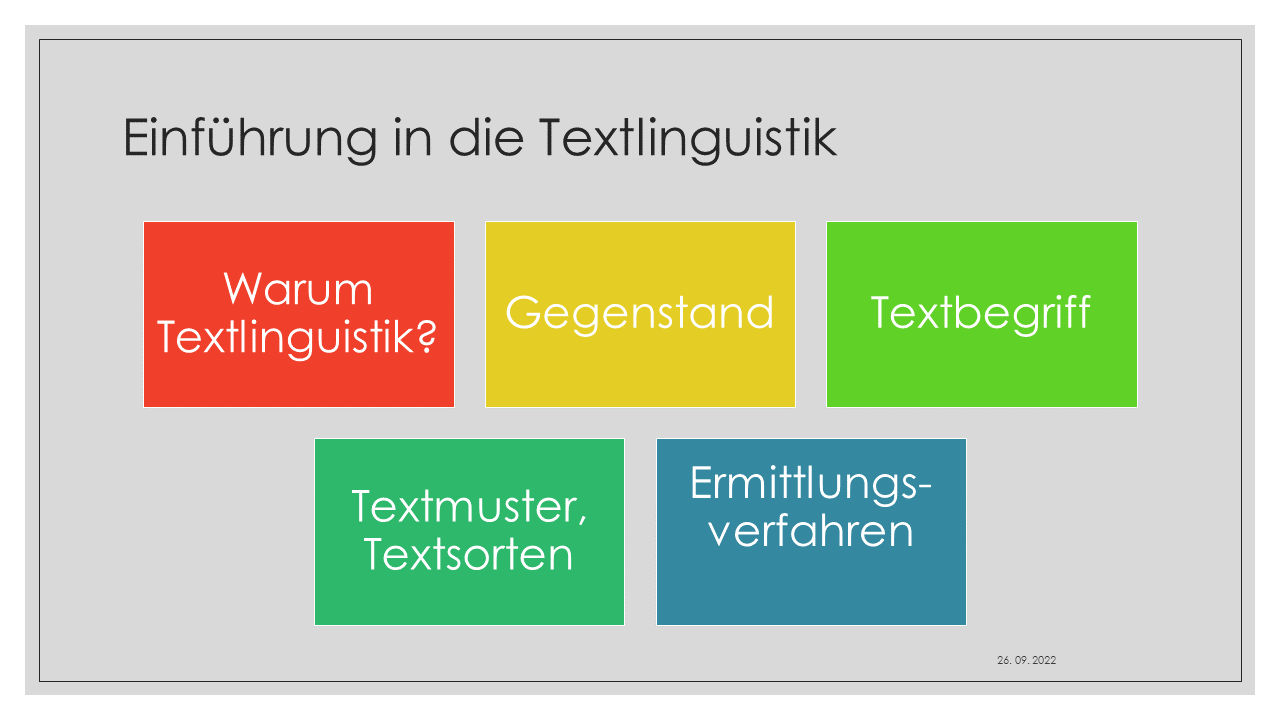
\includegraphics[width=1\textwidth,height=\textheight]{./pictures/Diapozitiv5.PNG}

In diesem Einführungskurs machen wir Sie mit grundlegenden Methoden zur
Erfassung von linguistischen Merkmalen in deutschen (und in einigen
Abschnitten auch mit slowenischen) Texten bekannt.

Unseren Kurs beginnen wir mit Frage, wozu wir überhaupt über Sprache
reden und \emph{zu welchem Zweck über Textlinguistik?}

Da sich mehrere Wissenschaften mit Sprache und folglich auch mit Texten
auseinandersetzen, ist es sinnvoll, Textlinguistik von anderen
wissenschaftlichen Disziplinen abzugrenzen, um den \emph{Gegenstand
\{Chapter~\ref{sec-gegenstand}\} der Textlinguistik} (als Bestandteil
der Systemlinguistik) besser erkennen zu können.

In jeder wissenschaftlichen Disziplin werden grundlegende Einheiten
definiert. In der Textlinguistik ist die sprachliche \emph{Äußerung} die
maßgebliche Basiseinheit. Wie jede linguistische Einheit, kann man
Äußerungen verschiedentlich definieren. Andere grundlegende Einheiten
der Textlinguistik, die in diesem Einführungsbuch definiert, beschrieben
und anhand von exemplarischen Analysen veranschaulicht werden, sind
\emph{Text, Textmuster und Textsorten}.\footnote{Dieses Buch wurde mit
  \texttt{Quarto} \url{https://quarto.org/docs/books/} zusammengestellt.}

Hinweise\footnote{Clipart von \url{https://www.clipartmax.com/}}:

Das ist eine Definition (rmdnote).

Das ist ein Tip oder eine Info (rmdtip).

Das ist ein Arbeitsvorschlag (rmdrobot).

Das ist der RStudio Logotyp (rmdrstudio).

Das ist eine Warnung (rmdwarning).

Das ist eine Fehlermeldung (rmderror).

\bookmarksetup{startatroot}

\hypertarget{sec-gegenstand}{%
\chapter{Gegenstand und Sinn der Textlinguistik}\label{sec-gegenstand}}

\hypertarget{gegenstand}{%
\section{Gegenstand}\label{gegenstand}}

Im Alltag, sei es privat oder im Beruf, verständigen wir uns vorrangig
mit Hilfe von mündlich oder schriftlich formulierten Texten. Will man
einen Text besser verstehen oder den Aufbau eines Textes durchschaubar
machen, ist es sinnvoll, ihn nach nachvollziehbaren Prinzipien und
Methoden in kleinere Einheiten zu zerlegen.

Die Sprachwissenschaft is allerdings nicht die einzige Wissenschaft, die
sich mit Texten auseinandersetzt.

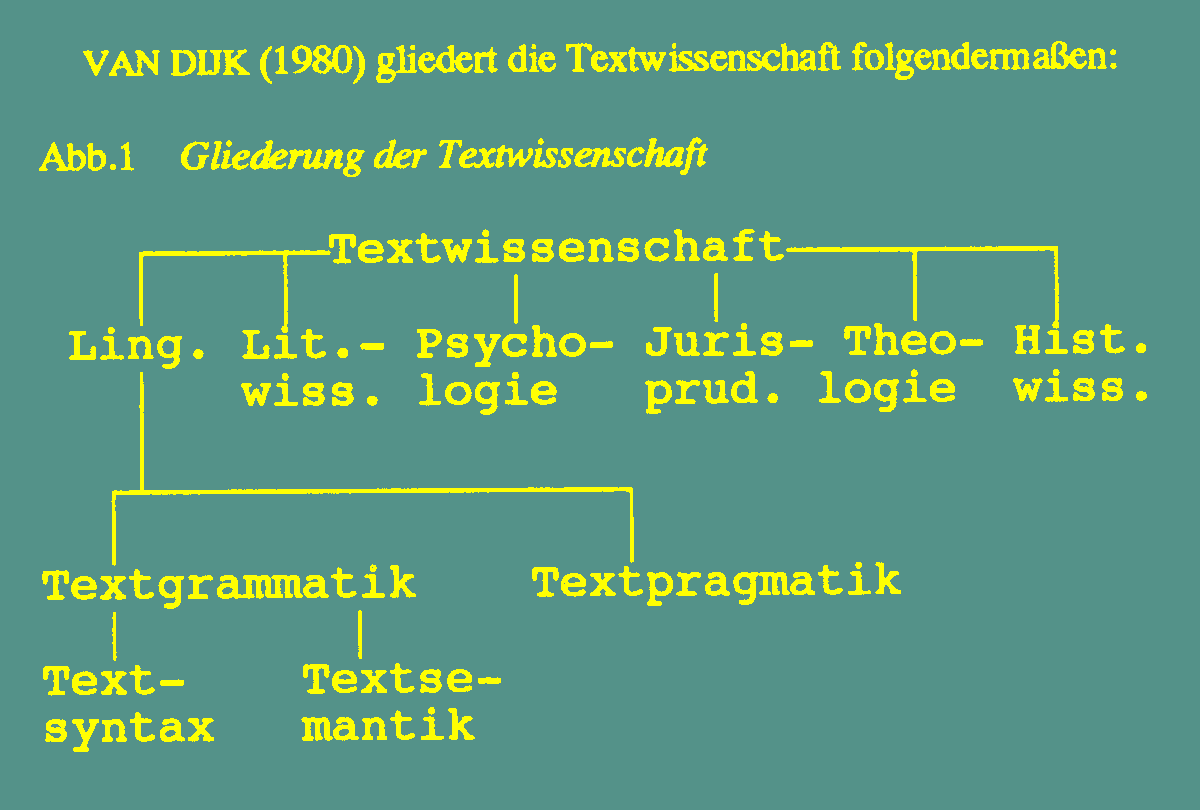
\includegraphics[width=0.75\textwidth,height=\textheight]{./pictures/textwissenschaften.png}

\begin{enumerate}
\def\labelenumi{\arabic{enumi}.}
\tightlist
\item
  Welchen \textbf{Zweck} erfüllen Texte im Rahmen der einzelnen
  Textwissenschaften?\\
\item
  Bei welchen Textwissenschaften sind die Texte auch das \textbf{Ziel}
  der wissenschaftlichen Auseinandersetzung?
\end{enumerate}

\textbf{Gegenstand} der Textlinguistik (Heinemann/Viehweger 1991:17):
Die Textlinguistik soll sich auf die Erforschung von Textstrukturen und
Textformulierungen beschränken, jeweils in ihrer Einbettung in
kommunikative, allgemein soziologische und psychologische Zusammenhänge
(interdisziplinärer Ansatz). - Der Text selbst bildet den primären und
originären Gegenstand der Wissenschaft vom Text, die zentrale Aufgabe
der Textlinguistik.

\textbf{Gegenstand} der Textlinguistik (Bußmann 1990: 779): Die
Textlinguistik ist eine sprachwissenschaftliche Disziplin, die sich mit
der Analyse satzübergreifender sprachlicher Regularitäten beschäftigt
und das Ziel hat, die konstitutiven Merkmale der sprachlichen Einheit
Text zu bestimmen und damit eine Texttheorie zu begründen.

\hypertarget{gesellschaftliche-relevanz}{%
\section{Gesellschaftliche Relevanz}\label{gesellschaftliche-relevanz}}

Welche \textbf{gesellschaftliche Relevanz} hat eine derart definierte
Textlinguistik?

Texte sind von grundlegender Bedeutung für die Existenz jeder
menschlichen Gesellschaft, da mit ihrer Hilfe gesellschaftliche
Beziehungen konstituiert werden. Die Fähigkeit zu angemessenem passiven
und/oder aktiven Umgang mit häufig auftretenden Textklassen ist
Voraussetzung dafür, dass jedes Mitglied einer Gesellschaft
sprachlich-kommunikativ tätig sein kann. Der Grad der effektiven und
angemessenen Beherrschung einer großen Anzahl kommunikativer Aufgaben
durch möglichst viele Mitglieder einer Gesellschaft hat daher Einfluss
auf das reibungslose Funktionieren kommunikativer Prozesse, mittelbar
auch auf den Zustand der sozialen Beziehungen in dieser Gesellschaft.

Mit Hilfe von Texten wird auch die begriffliche Verallgemeinerung der
Wirklichkeit ermöglicht, mentale Prozesse wahrnehmbar, verfügbar
(verschriftlicht und gespeichert!), Erfahrungen, Einstellungen und
Wertvorstellungen vermittelt. Texte stellen eine wesentliche Grundlage
für die Entwicklung und Vervollkommnung des Menschen und jeder
Gesellschaft dar.

Textlinguistische Darstellungen können Lesern Einsichten vermitteln in
charakteristische oder bewährte Organisationsformen bestimmter
Textklassen und in das Funktionieren bestimmter Texte in konkreten
gesellschaftlichen Situationen. Textvorkommen können vom Leser
selbständiger und bewußter durchdrungen werden.

Beispiel einer \textbf{Textdefinition} (Engel 1988:33)

\textbf{Texte} sind - Geflechte von Äußerungen - konnex - mit
nachvollziehbarer Struktur (?) - sortenspezifisch.

Der \textbf{Text} ist die umfangreichste und hierarchisch höchste
kommunikative Einheit, die aus inhaltlich zusammenhängenden
\emph{Äußerungen} besteht und eine nachvollziehbare und
sortenspezifische Struktur aufweist (Engel 1996: 33).

\hypertarget{grammatische-ebenen}{%
\section{Grammatische Ebenen}\label{grammatische-ebenen}}

In der Sprachwissenschaft hat sich eine längere Liste von
\textbf{Einheiten in Texten} etabliert, die man verschiedenen Bereichen
zuordnen kann. Hier sollen vor allem diejenigen Bereiche angeführt
werden, die gemeinsam die Grammatik einer Sprache umreißen.

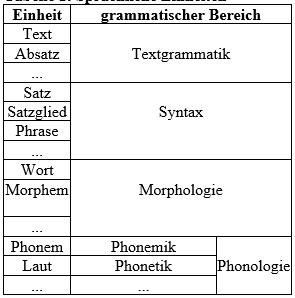
\includegraphics[width=0.6\textwidth,height=\textheight]{./pictures/grammatische_bereiche.png}

\hypertarget{uxe4uuxdferung}{%
\subsection{Äußerung}\label{uxe4uuxdferung}}

Eine \textbf{sprachliche Äußerung} kann als sinnvolle Lautfolge (oder
Schrifzeichenfolge) eines Textproduzenten zwischen zwei Pausen definiert
werden. Wie bei jedem sprachlichen Zeichen erfahren wir mit Hilfe der
Form einer Äußerung kommunikativ wichtige Aspekte ihrer Bedeutung, d.h.
semantische und pragmatische Merkmale. Einerseits kann die Form einer
Äußerung Auskunft darüber geben, \emph{was} (welchen Inhalt, welche
semantische Proposition) uns jemand mitteilen möchte, andererseits aber
auch, mit welcher \emph{Absicht} oder Zweck eine sprachliche Äußerung
erfolgt.

Inhalt + Absicht \textgreater\textgreater{}\\
Äußerung: Satzförmig \textless--\textgreater{} nicht-satzförmig

Sprachliche Äußerungen haben meist die Form (d.h. die Struktur, den
Aufbau) von satzförmigen bzw. satzartigen Konstruktionen (z.B.
Hauptsätze, Nebensätze, Infinitivgruppen), sie können aber auch
nicht-satzförmig realisiert sein (z.B. als Nominalphrase) (Engel 1996:
33). Die Form einer sprachlichen Äußerung hängt von der Absicht des
Kommunikationsteilnehmers, den zu übermittelnden semantischen Merkmalen
und verschiedenen situativen Umständen ab (den Adressaten der Botschaft,
den zeitlichen und räumlichen Kommunikationsverhältnisse u.a.). Die
systematische Ermittlung der Formaspekte sprachlicher Äußerungen und
ihrer Beziehungen zur Semantik und Pragmatik ist eine der wesentlichen
Aufgaben der Syntax. Im Rahmen der Syntax spielt der Satzbegriff eine
zentrale Rolle.

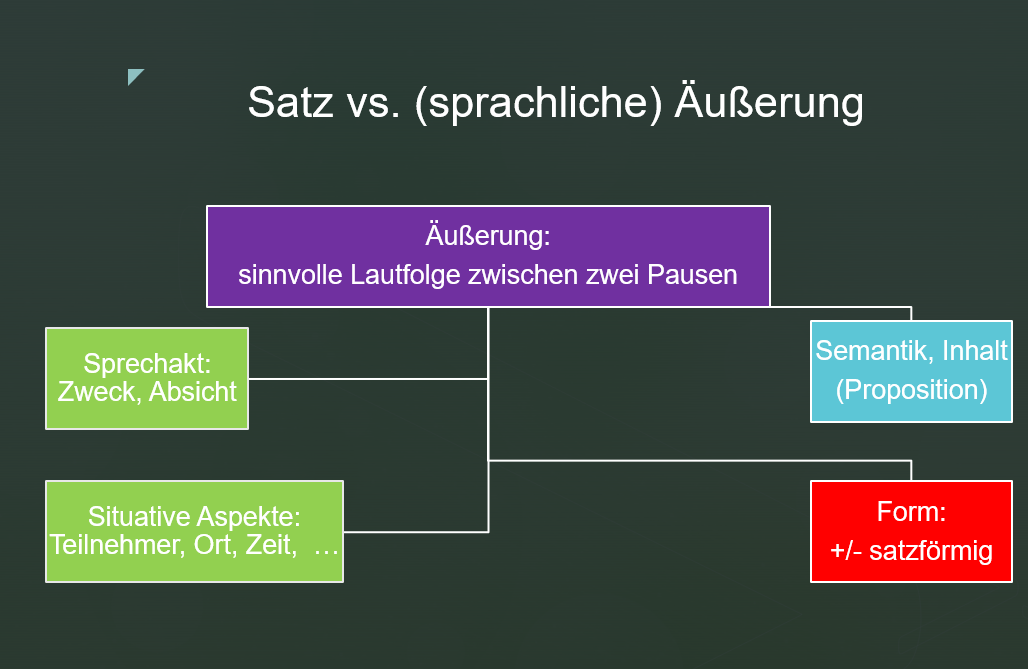
\includegraphics[width=1\textwidth,height=\textheight]{./pictures/aeusserung_vs_satz.png}

\textbf{Äußerungen} lassen sich als Laut- oder Schriftzeichenketten
definieren, die von einem Sprecher zwischen zwei Pausen produziert
werden und aus einem oder mehreren Sätzen bestehen können (Bußmann 1990:
52). Im Gegensatz zu Sätzen sind sie \emph{kommunikative} Einheiten und
gehören somit auf die Ebene der \emph{Performanz} oder Parole.
\textbf{Sätze} sind hingegen Einheiten des Sprachsystems und gehören
somit auf die Ebene der \emph{Kompetenz} oder Langue.

\hypertarget{prototypischer-satz}{%
\subsection{Prototypischer Satz}\label{prototypischer-satz}}

In mehreren Jahrzehnten intensiver syntaktischer Forschung wurden
mehrere hundert Satzdefinitionen vorgeschlagen. Trotz Gemeinsamkeiten
heben sie verschiedene Aspekte eines Satzes hervor. So wie bei vielen
anderen Begriffen in der Linguistik (und in der Natur überhaupt) ist
eine allgemein gültige Definition nicht möglich (vgl. etwa den
\emph{Wortbegriff}: Was ist ein Wort?)

Wir wollen in Anschluss an die deutsche Grammatik von (Engel 1996: 33)
einen \textbf{prototypischen Satz} definieren, und zwar mit folgenden
Eigenschaften:\\
- er soll eine finite Verbform enthalten;\\
- er soll sich dazu eignen, Sprechhandlungen eindeutig auszudrücken\\
- er soll kommunikativ selbständig sein und demnach kein unterordnendes
Element (z.B. einen Subjunktor) enthalten.

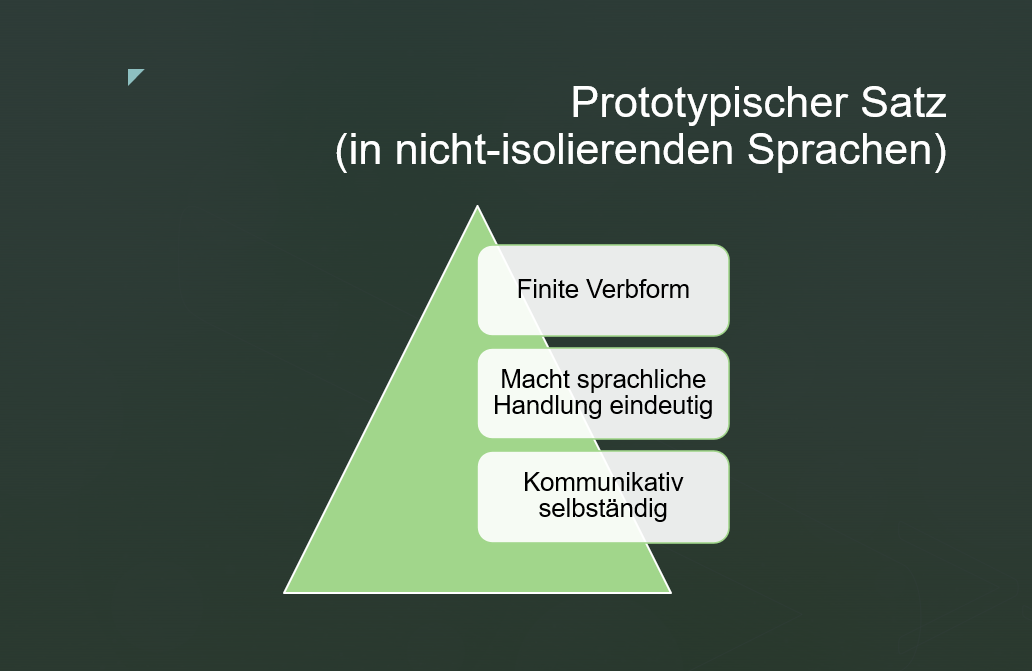
\includegraphics[width=1\textwidth,height=\textheight]{./pictures/satzdefinition.png}

Im Deutschen gibt es eine Reihe von sprachlichen Konstruktionen, die zu
verschiedenen Graden diese drei Eigenschaften aufweisen. Diese
Konstruktionen nennen wir satzförmige oder satzartige Konstruktionen
(sogenannte Haupt- und Nebensätze, Infinitiv- und
Partizipialkonstruktionen). Am anderen Ende dieser Skala stehen
nicht-satzartige Konstruktionen (z.B. Nominalphrasen).

Ordnen Sie die (mehr oder weniger satzförmigen) sprachlichen
Konstruktionen, die Sie im Textausschnitt identifizieren können, entlang
der im Rahmen der Syntax eingeführten \emph{Satzartigkeitsachse} an und
entscheiden Sie welche sprachlichen Konstruktionen \emph{Äußerungen}
darstellen!

\begin{quote}
Wie ich meine Muttersprache wiederfand\\
In Sibirien geboren, in Deutschland aufgewachsen: Unsere Autorin spricht
nur Deutsch, obwohl ihre Muttersprache Russisch ist. Heute macht sie
einen Sprachkurs -- und lernt die eigene Identität neu kennen.''
``„Ochen' khorosho'' -- sehr gut, lobt die Lehrerin, als ich ihr meine
kläglichen Versuche russischer Schreibschrift zeige, mit ihren vielen
Kurven und Häkchen. Ich lächele gequält und betrachte mein Werk, das
eher an die ersten Schreibversuche einer Grundschülerin erinnert als an
die Handschrift einer Neunundzwanzigjährigen. „Reine Übung'', sagt sie
mit breitem russischen Akzent, bevor sie uns die Hausaufgabe für die
kommende Woche aufbrummt. „Poka!{}``, sage ich, bevor ich den Laptop
zuklappe. Tschüss!
\end{quote}

Aus: Wie ich meine Muttersprache wiederfand (faz.net, 13.1.2022)

\hypertarget{identifikationsverfahren}{%
\section{Identifikationsverfahren}\label{identifikationsverfahren}}

Für die Identifizierung und Klassifizierung von Satzelementen verwenden
wir eine Reihe paradigmatischen und syntagmatischen Verfahren (Proben,
Tests).

\textbf{Identifikationsverfahren}

\textbf{1. Verschiebeprobe}\\
\textbf{2. Austauschprobe, Ersatzprobe}\\
\textbf{3. Eliminierungsprobe}\\
\textbf{4. Hinzufuegungsprobe}

Kombination aus Ersatz- und Verschiebeprobe:\\
\textbf{5. Fragetest}

Zusätzliche Tests:\\
6. Koordinationsprobe, Häufungsprobe, Akzentuierungsprobe mit Satz- oder
Kontrastakzent

\hypertarget{verschiebeprobe}{%
\subsection{Verschiebeprobe}\label{verschiebeprobe}}

Die \emph{Verschiebeprobe} wird auch Umstellprobe oder Permutationsprobe
genannt. Dieses Verfahren dient dazu, Konstituenten eines Satzes zu
ermitteln. Konstituenten des Satzes kann man in vielen Fällen mit der
Kategorie Satzglied gleichsetzen. Ein Ausdruck, der aus einem oder
mehreren Wörtern besteht, wird als Konstituente eines Satzes bezeichnet,
wenn er sich im Satz frei verschieben läßt.

(1a) Der Professor hält \emph{einen Vortrag über Textlinguistik}.\\
(1b) \emph{Einen Vortrag über Textlinguistik} hält der Professor.

Die unterstrichene Phrase in (1a) läßt sich frei im Satz verschieben,
z.B. an den Anfang des Satzes. Der Satz ist trotz der Verschiebung der
hervorgehobenen Phrase grammatisch richtig (1b). Daraus können wir
folgern, dass die hervorgehobene Phrase eine Konstituente des Satzes
ist.

Nun folgt ein Beispiel, in dem die hervorgehobene sprachliche Einheit
keine Satzkonstituente ist.

(2a) Der Professor hält einen Vortrag über Textlinguistik.\\
(2b) \textsuperscript{*}\emph{Einen} hält der Professor Vortrag über
Textlinguistik.

Das unterstrichene sprachliche Element in (2a) läßt sich nicht frei im
Satz verschieben. Stellt man es z.B. an den Anfang des Satzes, erhält
man einen ungrammatischen Satz (2b). Daraus folgern wir, daß das
unterstrichene sprachliche Element keine Konstituente des Satzes ist. Es
kann höchstens Teil einer Konstituente des Satzes sein.

\hypertarget{ersatzproben}{%
\subsection{Ersatzproben}\label{ersatzproben}}

\hypertarget{kommutationsprobe}{%
\subsubsection{Kommutationsprobe}\label{kommutationsprobe}}

Die \emph{Kommutationsprobe} ist eine Substitutions- oder
\emph{Ersetzungsprobe}. Dieses Verfahren dient dazu, Konstituenten mit
gleicher Funktion im Satz festzustellen. Lassen sich zwei oder mehrere
Ausdrücke füreinander austauschen, dann haben sie die gleiche Funktion
im Satz.

\begin{enumerate}
\def\labelenumi{(\arabic{enumi})}
\setcounter{enumi}{2}
\tightlist
\item
  \emph{Die Professorin} hält einen Vortrag über Textlinguistik. der
  Mann der Dozent die Frau Der da vorne die Studentin er sie \ldots{}
\end{enumerate}

Die untereinander stehenden Ausdrücke haben im Satz die gleiche
Funktion. Man sagt, sie kommutieren miteinander. Miteinander
kommutierende Ausdrücke bilden ein Paradigma (auch als System
bezeichnet).

\hypertarget{anaphorisierungsprobe}{%
\subsubsection{Anaphorisierungsprobe}\label{anaphorisierungsprobe}}

Die \emph{Anaphorisierungsprobe} ist eine Substitutions- oder
\emph{Ersetzungsprobe}. Dieses Verfahren dient dazu, die Satzgliedklasse
festzustellen, der eine Satzkonstituente angehört. Anaphern sind
Ausdrücke, die auf einen Ausdruck im Vortext hinweisen. Das Pronomen er
in (4) bezieht sich auf der Professor im davorstehenden Satz.

\begin{enumerate}
\def\labelenumi{(\arabic{enumi})}
\setcounter{enumi}{3}
\tightlist
\item
  \emph{Die Professorin} hält einen Vortrag über Textlinguistik.
  \emph{Sie} hat auch mehrere Bücher zu diesem Themenbereich
  veröffentlicht.
\end{enumerate}

Der Ausdruck \emph{die Professorin} kommutiert außerdem mit einer
speziellen Anapher, und zwar mit dem Pronomen \emph{sie}. Dies bedeutet,
dass man die Phrase \emph{die Professorin} in ein und demselben Satz
durch das Pronomen \emph{sie} ersetzen kann (5). Das ist deshalb
möglich, weil sie im Satz dieselbe Satzgliedfunktion haben (nämlich
Subjektfunktion).

\begin{enumerate}
\def\labelenumi{(\arabic{enumi})}
\setcounter{enumi}{4}
\tightlist
\item
  \emph{Die Professorin} hält einen Vortrag über Textlinguistik.
  \emph{Sie} \ldots{}
\end{enumerate}

Für jede Satzgliedklasse (Ergänzungsklasse) kann man im Prinzip eine
spezielle Anapher finden. Auf diese Weise ist eine
Satzgliedklassifizierung möglich. Die Anaphorisierungsprobe wirkt so wie
die Kommutationsprobe entlang der paradigmatischen Achse (y-Achse).

\hypertarget{fragewortprobe}{%
\subsection{Fragewortprobe}\label{fragewortprobe}}

Die \emph{Fragewortprobe} ist eine Ersetzungsprobe, bei der man aber
meist zusätzlich die Reihenfolge der Satzelemente verändert, da man das
Fragewort im Deutschen gewöhnlich an den Satzanfang stellt. Sie dient
wie die Anaphorisierungsprobe der Ermittlung der Satzgliedklasse. Eine
Konstituente des Satzes wird durch ein entsprechendes Fragewort ersetzt,
d.h. man versucht die betreffende Konstituente zu erfragen.

(6a) \emph{Die Professorin} hält einen Vortrag über Textlinguistik.\\
(6b) \emph{Wer} hält einen Vortrag über Textlinguistik?\\
(6c) Die Professorin hält einen Vortrag \emph{worüber}?\\
(6d) \emph{Worüber} hält die Professorin einen Vortrag?\\
(6e) (Die Professorin hält einen Vortrag) \emph{über Textlinguistik}.

Die Fragewortprobe besteht genau genommen aus zwei Tests:\\
(a) der Verschiebe- oder Umstellprobe (siehe 6d) und\\
(b) dem Einsetzen eines entsprechenden Fragewortes.\\
Sie ist also ein syntagmatischer Test (a), gleichzeitig aber auch ein
paradigmatischer (b). Deshalb wird vozugsweise eine Kommutations- oder
Anaphorisierungsprobe zur Identifizierung von Satzelementklassen
eingesetzt (außer in einigen Fällen, in denen die Fragewortprobe bessere
Einsichten bietet, z.B. bei adverbialen Bestimmungen der Folge, den
Konsekutivangaben).

\hypertarget{eliminierungsprobe}{%
\subsection{Eliminierungsprobe}\label{eliminierungsprobe}}

Die \emph{Eliminierungsprobe} (auch \emph{Weglassprobe} oder
\emph{Tilgungsprobe} genannt) dient zur Ermittlung von obligatorischen
und fakultativ auftretenden Konstituenten des Satzes. In der
Valenzgrammatik wird betont, daß die Unterscheidung zwischen Ergänzungen
und Angaben mit ihr nicht möglich ist.

(6a) Die Professorin hält einen Vortrag über Textlinguistik.\\
(6b) *Die Professorin hält über Textlinguistik.\\
(7a) Die Professorin spricht mit ihren Studierenden über
Textlinguistik.\\
(7b) Die Professorin spricht mit ihren Studierenden.\\
(7c) Die Professorin spricht über Textlinguistik.\\
(7d) Die Professorin spricht.

In (6b) sehen wir, daß das Verb halten obligatorisch eine
Akkusativergänzung verlangt (einen Vortrag), während das
bedeutungsähnliche Verb sprechen fakultative Ergänzungen aufweist (7).
Läßt man obligatorische (d.h. syntaktisch notwendige) Ergänzungen weg,
erhält man einen ungrammatischen Satz. Ist eine Ergänzung lediglich
fakultativ (d.h. syntaktisch nicht notwendig), bleibt der Satz
grammatisch richtig.

Manchmal wird die sogenannte \emph{Reduktionsprobe} von der
Tilgungsprobe unterschieden. Während bei der \emph{Tilgungsprobe} eine
beliebige Konstituente weggelassen wird, insofern der Satz dadurch nicht
ungrammatisch wird, können bei der \emph{Reduktionsprobe} auch
syntaktisch notwendige Konstituenten weggelassen werden. Während das
weggelassene Element nach der Tilgungsprobe nicht mehr zu rekonstruieren
ist, kann das weggelassene Element nach der Reduktionsprobe noch
rekonstruiert werden, d.h. dass der Hörer in der Lage ist, die
ausgelassene Konstituente zu ergänzen (Woellstein-Leisten et al. 1997:
16).

\begin{enumerate}
\def\labelenumi{(\arabic{enumi})}
\tightlist
\item
  {[}Das Wasser{]} kocht. / {[}Es{]} kocht.  * \_\_ kocht.
\item
  Hühner essen {[}Eier{]}, Menschen essen {[}Eier{]}.  Hühner essen
  \_\_, Menschen essen Eier.
\end{enumerate}

Ergibt sich wie in (2) eine elliptische Konstruktion, so wurde nur eine
Konstituente getilgt.

\hypertarget{hinzufuxfcgungsprobe}{%
\subsection{Hinzufügungsprobe}\label{hinzufuxfcgungsprobe}}

Die Hinzufügungsprobe (auch: Additionstest) ist das Gegenteil der
Tilgungsprobe oder Eliminierungsprobe. Durch Hinzufügung eines
sprachlichen Elements (eines Wortes, einer Phrase, eines Satzes) können
wir feststellen, ob ein sprachliches Element mit einer Satzkonstruktion
syntaktisch kompatibel (verträglich) ist.

\begin{enumerate}
\def\labelenumi{(\arabic{enumi})}
\setcounter{enumi}{2}
\tightlist
\item
  Die Studentin fährt.\\
\item
  Die Studentin spricht.\\
\item
  Die Studentin fährt {[}an die Uni{]}.\\
\item
  Die Studentin spricht \textsuperscript{*}{[}an die Uni{]}.
\end{enumerate}

Die satzförmigen Äußerungen (3) und (4) sind wohlgeformt. In (5) und (6)
fügen wir die Präpositionalphrase \emph{an die Uni} zu den bereits
bestehenden Satzkonstruktionen. Wir erkennen, dass die
Präpositionalphrase nur mit (5) syntaktisch kompatibel ist, mit (6)
dagegen nicht. Das liegt daran, dass das Verb \emph{fahren} in (5) die
Hinzufügung einer Phrase, mit der wir das (geographisch bestimmbare)
Ziel einer Bewegung angeben, erlaubt ist. Das Verb \emph{sprechen} in
(6) gehört dagegen zu einer anderen Verbklasse. Es ist kein
\emph{Fortbewegungsverb}, sondern ein \emph{Verb des Meinens und
Sagens}. Daher ist die Hinzufügung einer Phrase, in der der Zielort
angegeben wird, nicht erlaubt.

Dass die beiden Verben unterschiedlichen Klassen (mit verschiedener
Semantik und Syntax) angehören, wird durch die folgenden Beispiele
erhärtet.

\begin{enumerate}
\def\labelenumi{(\arabic{enumi})}
\setcounter{enumi}{6}
\tightlist
\item
  Die Studentin fährt {[}zu ihren Freundinnen{]}. (Zielort)\\
\item
  Die Studentin spricht {[}zu ihren Freundinnen{]}. (Adressaten)\\
\item
  Die Studentin fährt {[}mit ihren Freundinnen{]}. (Begleitung)\\
\item
  die Studentin spricht {[}mit ihren Freundinnen{]}. (Adressaten)
\end{enumerate}

Hier erhebt sich die Frage: wenn die Studentin zu ihren Freundinnen
spricht, sind die Freundinnen dann das Ziel der Handlung
\emph{sprechen}?

Hier fällt ein semantischer Unterschied zwischen dem ``Ziel'' des Verbs
\emph{fahren} und dem des Verb \emph{sprechen} auf: wenn die Studentin
fährt, verändert sie ihren Standort (von Punkt A nach Punkt B), wenn sie
jedoch spricht, ist damit nicht gesagt, dass sie ihren Standort
wechselt. Deshalb unterscheiden wir gewöhnlich zwischen den semantischen
Klassen \{Ziel\} und \{Adressat\}. Erstere ist mit Fortbewegungsverben
kompatibel, letztere dagegen mit Verben des Meinens und Sagens. Die
Beispiele zeigen also, dass man die semantische Klasse \{Ziel\} nur mit
dem Fortbewegungsverb \emph{fahren} kombinieren kann, nicht mit dem Verb
\emph{sprechen}. Die semantischen Unterschiede haben demnach
Konsequenzen in der syntaktischen Form des Satzes.

\hypertarget{koordinationsprobe}{%
\subsection{Koordinationsprobe}\label{koordinationsprobe}}

Wenn sich zwei oder mehrere Elemente eines Satzes durch eine
koordinierende Konjunktion (wie \emph{und} oder \emph{oder}) verbinden
lassen, bilden sie eine Konstituente.

\begin{enumerate}
\def\labelenumi{(\arabic{enumi})}
\tightlist
\item
  {[}{[}Die Studierenden{]} und {[}Professor\_innen{]}{]} machen eine
  gemeinsame Exkursion.\\
\item
  {[}Der eine freut sich{]} und {[}der andere ärgert sich{]}.\\
\item
  eine {[}reizvolle{]} und {[}intelligente{]} Frau
\end{enumerate}

\hypertarget{huxe4ufungsprobe}{%
\subsection{Häufungsprobe}\label{huxe4ufungsprobe}}

Bestimmte Ausdrücke (etwa Partikeln) können gehäuft werden, d.h. sie
können gleichzeitig im Satz auftreten, ohne daß sie durch eine
koordinierende Konjunktion (z.B. und) miteinander verbunden werden
könnten, ohne daß sie frei im Satz verschiebbar wären (wie etwa
Konstituenten im Satz) oder gemeinsam im Satz verschiebbar wären (wie
etwa Bestandteile von Konstituenten).

\begin{enumerate}
\def\labelenumi{(\arabic{enumi})}
\tightlist
\item
  Der Junge hat ja eben keinen Hunger.\\
\item
  *Der Junge hat ja und eben keinen Hunger.\\
\item
  *Ja hat der Junge eben keinen Hunger.\\
\item
  *Eben hat der Junge ja keinen Hunger.\\
\item
  *Ja eben hat der Junge keinen Hunger.
\end{enumerate}

\hypertarget{akzentuierung}{%
\subsection{Akzentuierung}\label{akzentuierung}}

Durch entsprechende Akzentuierung (Satzakzent, Kontrastakzent)) und
Herstellung eines entsprechenden Kontextes (z.B. einer tatsächlich im
Text vorkommenden oder nur gedachten allgemeinen oder einer spezifischen
Fragestellung) zeigt sich erst, ob eine bestimmte Satzform in einer
Sprache möglich ist. Die Großschreibung in den folgenden Beispielen
indiziert den Satz- bzw. den Kontrastakzent.

\begin{enumerate}
\def\labelenumi{(\arabic{enumi})}
\tightlist
\item
  Kontext: \emph{Heute Abend findet das Queen-Konzert statt}.\\
  (gedachte spezifische Frage: Wer nimmt den Wagen, da wir nur einen
  haben?) \emph{Den Wagen nehme ICH}. (Kontrastakzent)\\
\item
  Kontext (allgemeine Frage von A): \emph{Was ist denn hier passiert?} -
  B: \emph{Ich bin mit unserem Wagen in ein VerKEHRSschild geknallt}.
  (Satz- oder Fokusakzent)
\end{enumerate}

\hypertarget{identifizierungsprobleme}{%
\subsection{Identifizierungsprobleme}\label{identifizierungsprobleme}}

Nachdem vier grundlegende Verfahren zur Identifizierung von
Satzkonstituenten und ihrer Rolle im Satz vorgeführt wurden, soll in den
nächsten Absätzen einige der möglichen \emph{Schwierigkeiten} gezeigt
werden, die \emph{bei der Verwendung dieser Verfahren} auftreten können.

Die \emph{Verschiebeprobe} liefert beispielsweise nicht in allen Fällen
eindeutige Ergebnisse, d.h. man kann mit ihr nicht immer eindeutig
nachweisen, daß ein sprachliches Element keine Konstituente des Satzes
ist. In (3) ist dieses Problem veranschaulicht.

(3a) Die Professorin hält einen Vortrag {[}über Textlinguistik{]}.\\
(3b) {[}Über Textlinguistik{]} hält die Professorin einen Vortrag.

Die hervorgehobene Präpositionalphrase in (3a) läßt sich frei im Satz
verschieben, z.B. an den Anfang des Satzes. Ist diese Phrase dann etwa
auch eine Konstituente des Satzes? Die \emph{Verschiebeprobe} legt dies
nahe. Dagegen spricht allerdings das \emph{Dependenzprinzip} (ein
semantisch begründetes Prinzip), denn man kann zeigen, daß die
Präpositionalphrase über Textlinguistik vom Nomen \emph{Vortrag} regiert
(verlangt) wird und nicht vom Verb \emph{halten}.

Das Nomen \emph{Vortrag} fordert folgende Ergänzungen: - eine Person,
die vorträgt (also spricht),\\
- und einen Gegenstand, der von der Person vorgetragen wird.\\
Die handelnde Person wird als Satzsubjekt am Satzanfang genannt und
braucht daher nicht als Genitivattribut in der Nominalphrase wiederholt
zu werden, der Gegenstand des Vortrags in der Präpositionalphrase.

Das Verb \emph{halten} fordert - ebenfalls eine handelnde Person (als
Subjekt im Satz)\\
- und einen Gegenstand, fordert allerdings im Gegensatz zum Nomen
\emph{Vortrag}, daß der Gegenstand als Nomen im Akkusativkasus
realisiert wird: vgl. (4) mit (5)

\begin{enumerate}
\def\labelenumi{(\arabic{enumi})}
\setcounter{enumi}{3}
\tightlist
\item
  \emph{halten} \textless(Person: nom), (Gegenstand: akk)\textgreater{}
\item
  \emph{Vortrag} \textless(Person: gen), (Gegenstand: prp)\textgreater.
\end{enumerate}

Die Präpositionalphrase \emph{über Textlinguistik} kann demnach nicht
der geforderte Gegenstand zum Verb \emph{halten} sein, sondern nur die
Nominalphrase \emph{einen Vortrag}, die im Akkusativ steht.

Ersetzt man die Präpositionalphrase \emph{über Textlinguistik} in (3)
durch eine Nominalphrase im Akkusativ \emph{die Textlinguistik} ,
entstünde ebenfalls ein ungrammatischer Satz.

Die \emph{Kommutationsprobe} (d.h. der Austausch der Präpositionalphrase
durch eine Nominalphrase) zeigt somit, zwischen welchen Teilen des
Satzes engere Abhängigkeitsbeziehungen bestehen.

Das \emph{Abhängigkeitsprinzip} legt demnach über die Valenzbeziehungen
zwischen den Satzelementen nahe, dass die Präpositionalphrase \emph{über
Textlinguistik} keine unmittelbare Konstituente des Satzes, sondern
lediglich eine unmittelbare Konstituente der Nominalphrase \emph{einen
Vortrag} ist. Einen Teil einer Satzkonstituente (oder eines Satzgliedes)
nennt man auch ein Attribut.

Die \emph{Eliminierungsprobe} unterstützt in diesem Fall das Ergebnis,
das die Kommutationsprobe erbracht hat, denn sie zeigt ebenfalls, dass
die ausgelassene Nominalphrase ein obligatorischer Bestandteil des
Satzes ist, während dies für die Präpositionalphrase nicht zutrifft:
Lässt man nämlich \emph{einen Vortrag} in (3) aus, dann erhalten wir
einen ungrammatischen Satz (3c).

(3a) Die Professorin hält einen Vortrag {[}über Textlinguistik{]}. (3c)
*{[}Über Textlinguistik{]} hält die Professorin.

Die Nominalphrase \emph{einen Vortrag} (samt Präpositionalattribut
\emph{über Textlinguistik}) ist somit eine obligatorische Ergänzung des
Verbs. Daß die Ergänzung \emph{einen Vortrag} obligatorisch im Satz mit
dem Verb halten vorkommen muß, zeigt die \textbf{Eliminierungsprobe}.

Die semantischen und syntaktischen Verhältnisse in (3) liegen allerdings
noch komplizierter, denn bei genauerer Überlegung sieht man, daß die
Nominalphrase \emph{einen Vortrag} und das Verb \emph{halten} zusammen
das Prädikat des Satzes bilden, d.h. semantisch eine Einheit bilden.
Beide Varianten haben die Grundbedeutung: ``\emph{etwas vor einem
Auditorium sprachlich vermitteln}''. Das kann man nachweisen, indem man
beide Ausdrücke durch einen Ausdruck ersetzt, und zwar \emph{einen
Vortrag halten} durch \emph{vortragen}. Wenn \emph{einen Vortrag} und
\emph{halten} nun gemeinsam das Prädikat bilden, könnte man die
Präpositionalphrase \emph{über Textlinguistik} dennoch für eine
unmittelbare Konstituente des Satzes halten. Dann wäre auch
verständlich, warum sich die Präpositionalphrase frei im Satz
verschieben lässt.

Versucht man nun das einfache Verb \emph{vortragen} in (3) statt des
komplexen Ausdrucks \emph{einen Vortrag halten} einzusetzen, stößt man
jedoch auf Schwierigkeiten. Die beiden Varianten haben zwar dieselbe
Grundbedeutung (4), das einfache Verb ist jedoch nicht in (3)
einsetzbar.

(3a) Die Professorin hält einen Vortrag über Textlinguistik. (3d) *Die
Professorin trägt über Textlinguistik vor. (3e) Die Professorin trägt
einen Text vor.

Das einfache Verb ist nicht in (3) einsetzbar, weil es eine andere
syntaktische Valenz hat. Es fordert nämlich (wie das Verb \emph{halten})
keine Präpositionalphrase als Objekt (3d), sondern eine Nominalphrase
mit einem Nomen im Akkusativ \emph{Text} (3e). Die Äußerung (3a) zeigt
im Vergleich mit (3e) auch einen kleinen, aber wichtigen semantischen
Unterschied, der parallel zum syntaktischen verläuft: Verwendet man das
komplexe Prädikat \emph{einen Vortrag halten}, dann nennt man in der
Präpositionalphrase den Bereich, über den gesprochen wird. Verwendet man
hingegen das einfache Verb \emph{vortragen}, dann nennt man im
Akkusativkasus den Gegenstand und nicht den Bereich. Der Gegenstand in
(3e) ist ein Text, d.h. eine inhaltlich zusammenhängende Folge von
Äußerungen. Dieser Text kann schriftlich fixiert sein und damit auch in
konkreter Form auf Papier vorliegen. Der Bereich ist ein abstrakterer
Gegenstand als der Text. Er ließe sich allenfalls mit einer Skizze
konkretisieren.

Der Vergleich von (3a) mit (3f) ergibt noch einen weiteren syntaktischen
und gleichzeitig semantischen Unterschied.

(3a) Die Professorin hält einen Vortrag über Textlinguistik. (3f) Die
Professorin trägt einen Text über Textlinguistik vor.

Das einfache Verb \emph{vortragen} hat zwar dieselbe Grundbedeutung wie
\emph{einen Vortrag halten} (siehe oben), aber das komplexe Prädikat
\emph{einen Vortrag halten} enthält noch ein weiteres semantisches
Merkmal, nämlich das Merkmal \emph{Gegenstand}. Dieses Merkmal wird
durch das Nomen \emph{Vortrag} realisiert. Der Vortrag läßt sich ja
genau genommen paraphrasieren als ``\emph{Text, der vorgetragen wird}''.
Dies bedeutet, daß der Begriff ein Text in das Wort Vortrag
hineinverlegt (inkorporiert) worden ist. Demnach ist es richtiger, das
komplexe Prädikat einen Vortrag halten mit dem komplexen Prädikat einen
Text vortragen zu paraphrasieren (3g):

(3a) Die Professorin hält einen Vortrag über Textlinguistik. (3g) Die
Professorin trägt einen Text über Textlinguistik vor.

Die Äußerung (3a) mit dem Nominalisierungsverbgefüge \emph{einen Vortrag
halten} entpuppt sich damit als verkürzender Ausdruck für das
morphologisch komplexe (und außerdem auch trennbare) Verb
\emph{vortragen} und dessen Akkusativobjekt \emph{einen Text}. Will der
Sprecher lediglich den Bereich nennen, über den die Rede ist, verwendet
er das Nominalisierungsverbgefüge. Wenn er aber den konkreten
Text(gegenstand) nennen will, verwendet er das komplexe Verb vortragen
(z.B. ein Gedicht vortragen). Die beiden Ausdrücke einen Vortrag über
etwas halten und etwas über etwas vortragen sind demnach nur scheinbar
völlig bedeutungsgleich, was sich durch ihre unterschiedliche
Verwendbarkeit zeigt.

Was hat die Untersuchung von Äußerung (3) nun für die Lösung der Frage
gebracht, ob die Präpositionalphrase \emph{über Textlinguistik} in (3a)
eine Konstituente des Satzes ist oder nicht? Mein Lösungsvorschlag ist
folgender:

Berücksichtigt man das \textbf{Dependenzprinzip} (und die damit
zusammenhängenden Subkategorisierungsrahmen des Verbs \emph{halten} und
des Nomens \emph{Vortrag}) ist es angemessener, davon auszugehen, dass
die Präpositionalphrase \emph{über Textlinguistik} semantisch und
syntaktisch direkt vom Nomen \emph{Vortrag} abhängig ist und lediglich
aufgrund der besonders engen semantisch-syntaktischen Verbindung
zwischen dem Verb \emph{halten} und \emph{Vortrag} syntaktisch weder
eindeutig als Attribut noch als Satzkonstituente eingeordnet werden
kann.

In (3a) ist die Präpositionalphrase zwar direkt abhängig vom Nomen
\emph{Vortrag} (und demnach dessen Attribut); da aber \emph{einen
Vortrag halten} eine semantische Einheit bildet und in Satz (3a) als
komplexes Prädikat auftritt, scheint es folgerichtig, die vom komplexen
Prädikat abhängige Präpositionalphrase auch als Konstituente des Satzes
und damit als Satzglied zu behandeln. Die Präpositionalphrase hat somit
Zwitterstatus: gleichzeitig Attribut und Satzglied.

In (3g) hat das Verb \emph{vortragen} im Gegensatz zum Verb
\emph{halten} in (3a) volle lexikalische Bedeutung und nicht lediglich
Funktionsverbcharakter oder Nominalisierungsverbcharakter (d.h.
\emph{halten} hat vor allem eine strukturelle Funktion, die darin
besteht, die zweite Stelle im Aussagesatz durch einen Ausdruck mit
Finitheitsmerkmalen zu besetzen). Die Nominalphrase \emph{einen Text}
mit einem Nomen im Akkusativ ist abhängig von einem Vollverb, als
Ergänzung des Verbs einzuordnen (d.h. als eine valenzbedingte Art von
Satzglied) und außerdem Konstituente des Satzes, da sie sich im Satz
frei verschieben läßt. Die Präpositionalphrase \emph{über
Textlinguistik} ist abhängig von einer Konstituente des Satzes, nämlich
von dem Akkusativobjekt \emph{einen Text} und daher lediglich Attribut.
Sie ist unmittelbare Konstituente des Akkusativobjekts und nur eine
indirekte Konstituente des Satzes.

Die beiden folgenden Dependenzdiagramme sollen dies veranschaulichen: In
(3a) steht das Nomen \emph{Vortrag} auf erster Abhängigkeitsstufe, die
Präpositionalphrase \emph{über Textlinguistik} auf zweiter und dritter
Abhängigkeitsstufe. Die ``Abhängigkeitsdistanz'' beträgt somit 1. In
(3g) steht das Verb \emph{vortragen} (das dieselbe Grundbedeutung hat
wie das Nomen \emph{Vortrag}) auf nullter Abhängigkeitsstufe, die
Präpositionalphrase \emph{über Textlinguistik} auf zweiter und dritter
Abhängigkeitsstufe. Die ``Abhängigkeitsdistanz'' ist also größer als in
(3a) und beträgt 2. Die Präpositionalphrase ist in (3a) nur indirekt
abhängig vom regierenden Verb \emph{halten}, direkt abhängig dagegen vom
regierenden Nomen \emph{Vortrag}, das mit dem Verb \emph{vortragen} in
(3g) stammgleich und von der Grundbedeutung her damit äquivalent ist.
Die Präpositionalphrase ist in (3g) nur indirekt abhängig vom
regierenden Verb \emph{vortragen}, direkt abhängig dagegen vom
regierenden Nomen \emph{Text}. Das Nomen \emph{Vortrag} hat zwar wie das
Verb vortragen eine gemeinsame Bedeutungskomponente (``\emph{etwas vor
einem Auditorium sprachlich vermitteln}''), daneben aber auch noch die
Bedeutungskomponente ``\emph{Text}''. Durch diese zusätzliche
Bedeutungskomponente ist es ein ausgezeichneter Kandidat für die
Objektstelle des Verbs \emph{vortragen}.

\begin{enumerate}
\def\labelenumi{\arabic{enumi}.}
\tightlist
\item
  Was ist eine sprachliche Äußerung?\\
\item
  Wie haben wir den prototypischen Satz definiert?\\
\item
  Welches Verhältnis besteht zwischen Äußerungen und Sätzen?\\
\item
  Welche syntaktischen Mittel können laut (Eisenberg 1994) unterschieden
  werden?\\
\item
  Welche (syntaktischen) Identifikationsverfahren haben wir im
  Unterricht eingeführt?\\
\item
  Zeigen Sie an einem oder zwei geeigneten Textbeispielen den
  Unterschied zwischen kommunikativer Funktion, syntaktischer Funktion
  und Bedeutung!\\
\end{enumerate}

Lesen Sie den Text über den Rapper \emph{Capital Bra}
(\url{https://www.zdf.de/nachrichten/heute/das-phaenomen-capital-bra-100.html})!
Sehen Sie sich den Video-Beitrag (mit Untertiteln an)!
\emph{YouTube}-Video der Sendung \emph{Germania} über \emph{Capital
Bra}: \url{https://www.youtube.com/watch?v=7_oNPNvjphs}

Beschreiben Sie, welchen Eindruck Sie beim Lesen von der Sprache in den
beiden Texten erhalten haben? Können Sie Unterschiede zwischen den
beiden Texten erkennen? \emph{Wie} wird gesprochen bzw. geschrieben?

Zur computergestützen Textanalyse verwenden wir nun \emph{Voyant Tools}:
\url{https://voyant-tools.org/}. Adresse des Tutorials:
\url{https://voyant-tools.org/docs/\#!/guide/tutorial}.

Wir ``füttern'' das Programm mit beiden Texten (\emph{ZDF}-Beitrag,
Untertitel zum \emph{YouTube}-Video). Die Daten sollen uns bei unserer
stilistischen Analyse behilflich sein.

Wir erhalten mehrere Angaben und Darstellungen von \emph{Voyant Tools}:
z.B.\\
1. \emph{Wortwolke} (Cirrus): Welche (inhaltlich relevanten) Wortformen
kommen im ZDF-Text am häufigsten vor, welche in den
Germania-Untertiteln? Wie erklären Sie sich die Unterschiede? Schauen
Sie sich auch die \emph{Trends}-Darstellung an!\\
2. Haben Sie beim Lesen noch \emph{weitere Unterschiede} in der Wortwahl
bemerkt, die in den beiden Bilddarstellungen nicht sichtbar sind?\\
3. \emph{Dokumentlänge}: Wie viele \emph{Äußerungen} umfassen die beiden
Texte? Welcher ist länger? Kann man den Unterschied mit Hilf der
syntaktischen Einheit \emph{Satz} beschreiben?\\
4. \emph{Wortschatzdichte} (lexikalische Diversität): In welchem der
beiden Texte werden mehr unterschiedliche Wortformen verwendet? In
welchem der beiden werden öfters dieselben Wortformen benutzt?\\
5. \emph{Phrasen}: Welche Wortverbindungen werden in dem einen oder
anderen Text wiederholt verwendet?\\
6. \emph{Korrelationen}\footnote{``The correlation coefficient is
  calculated by comparing the relative frequencies of terms (relative to
  each document for the corpus or relative to each segment of document).
  A coefficient that approaches 1 indicates that values correlate
  positively, they rise and fall together. A coefficient that approaches
  -1 indicates that values correlate negatively, frequencies rise for
  one term as it drops for the other. Coefficients that approach 0
  indicate little correlation, positive or negative.'' -
  \url{https://voyant-tools.org/docs/\#!/guide/correlations}}
(Zusammenhänge): Welche Wörter kommen in dem einen oder anderen Text
gemeinsam vor (hohe Korrelation + Signifikanz kleiner als 0,05)?

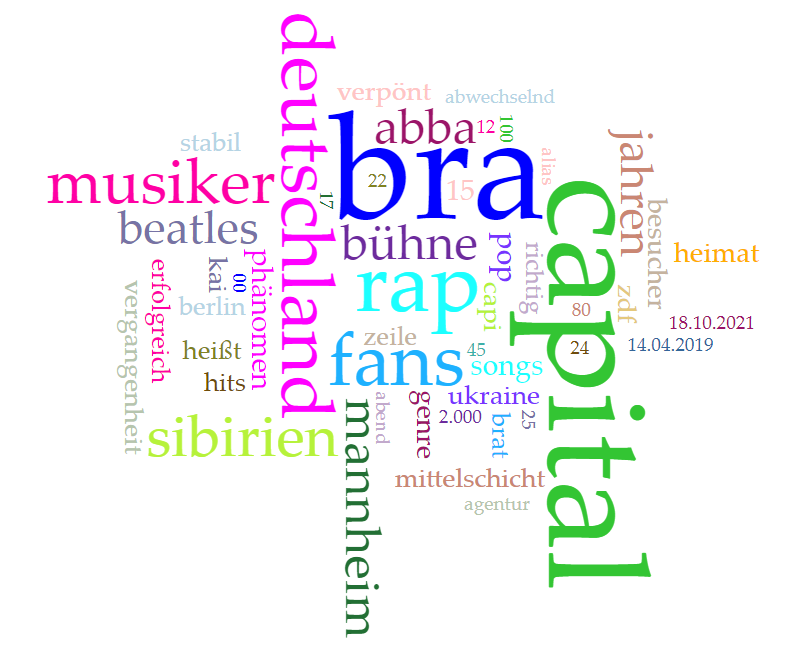
\includegraphics[width=1\textwidth,height=\textheight]{./pictures/capital_bra_untertitel.png}

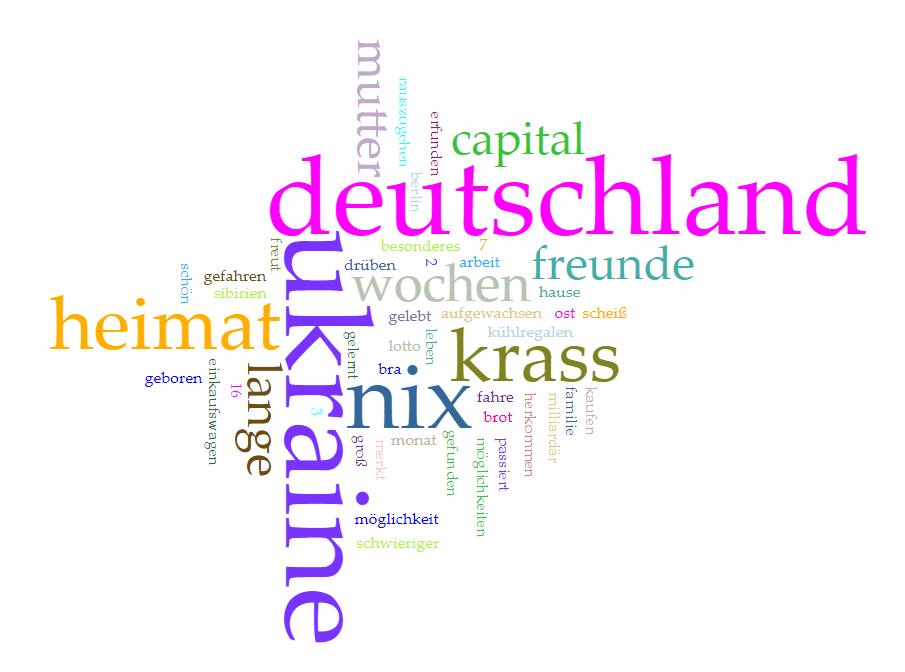
\includegraphics[width=1\textwidth,height=\textheight]{./pictures/capital_bra_zdf.png}

\textbf{Text (ZDF)}:

\begin{verbatim}
Das Phänomen Capital Bra - Erfolgreicher als die Beatles und Abba
Datum: 14.04.2019 15:00 Uhr
Aus Sibirien in die deutsche Hitparade: Capital Bra gilt als derzeit erfolgreichster Vertreter des Deutschraps. Einst war er provokant, doch längst ist er kommerziell erfolgreich.
Es ist ein historischer Moment, ein Stück deutscher Musikgeschichte - daran will zumindest der Hallensprecher gar keinen Zweifel aufkommen lassen. Mehr Nummer-eins-Hits als die Legenden Abba und Beatles habe der Künstler bundesweit eingesammelt, heißt es vor dem Konzert von Deutschlands derzeit wohl erfolgreichstem Rapmusiker in Mannheim. Dann kommt Vladislav Balovatsky alias Capital Bra auf die Bühne und bringt mehr als 2.000 Jugendliche zum Singen und Tanzen. Der Mann mit der Mütze ist ein Phänomen - vom "Wachwechsel im Pop" schreibt bereits das Fachmagazin "Rolling Stone".
Junge Fans
Für Capital Bra ist Mannheim die erste Station seiner Tournee, die den 24-jährigen Berliner kreuz und quer durch Deutschland führt, außerdem nach Wien und Zürich. Textsicher singen die Besucher an diesem Abend Zeile für Zeile mit, ziehen die Endvokale wie der Sänger auf der Bühne: "Weit und breit keine Gegnaaaa, komm wir wechseln das Themaaaa, ich will 22-Zoll-Rädaaaa, und die Sitze aus Ledaaaa". Die Songs ähneln einander, es geht um Aufsteigerträume und dosierte Kritik am Staat sowie um Mädchen, Mode, Maschinen. In rund 80 Minuten spielt Capital Bra seine Hits, darunter "Cherry Lady" und "Neymar".
    "Das ist richtig stabil." Kai, ein Fan
Den meisten gefällt es. "Das ist richtig stabil", sagt der 17-jährige Kai aus Heidelberg. Und die 15-jährige Jana aus Karlsruhe schwärmt: "Also, ich feiere den." Fast pausenlos filmen sie abwechselnd den Musiker und sich mit dem Smartphone. Ruhelos tanzt Capital Bra, musikalisch unterstützt von einem DJ, auf der Bühne hin und her - im Dresscode der Straßengang: lässige Kleidung und Baseballcap. Auf seine Frage "Was geht ab, Bratans und Bratinas?", wie der Musiker seine Fans nennt, folgen "Capi Capi"-Sprechchöre. Es ist für die meisten der jungen Besucher eine ausgelassene Feier - und draußen wartet der Vater im Auto.
Kleinkriminelle Vergangenheit
Der in Sibirien geborene und in der Ukraine aufgewachsene Capital Bra steht für viele stellvertretend für den einst provokanten Straßenrap, der den Weg aus prekären Plattenbauten in situierte Vorstadtvillen gefunden hat. Die Musikform sei längst in der Mitte der Gesellschaft angekommen, sagt Marcus Kleiner, Professor für Medien- und Kommunikationswissenschaft an der SRH Hochschule der populären Künste Berlin. Fans seien vor allem 12- bis 25-Jährige.
Capital Bra über seine neue Heimat Deutschland
Capital Bra wurde in Sibirien geboren, ist in der Ukraine aufgewachsen - und kam mit sieben Jahren nach Deutschland. Wie das für ihn war, hat er bereits vor zwei Jahren den Kollegen von Germania erzählt - einem Format von funk, dem gemeinsamen Jugendangebot von ARD und ZDF. Deutschland sei längst seine Heimat, sagte Capital Bra damals. "Ich bin hier groß geworden, hab hier die Sprache gelernt, meine Freunde sind hier, meine Familie ist hier." Hier geht es zum ganzen Video auf YouTube.
"Bra" steht für "Brat", das russische Wort für Bruder. "Brat" heißt auch ein russischer Kultfilm über einen Außenseiter. Der Rapper, der aus der Kälte kam, zog mit sieben Jahren mit seiner Mutter nach Berlin-Hohenschönhausen und wurde durch die Veranstaltung "Rap am Mittwoch" bekannt. Der Vergleich mit Abba und den Beatles hinkt indes - im digitalen Zeitalter entstehen Hitparaden ganz anders als damals.
Der Reiz bestehe darin, dass Capital Bra aus seiner kleinkriminellen Vergangenheit und anderen kontroversen Themen aus seinem Leben kein Hehl mache und die Entwicklung vom "Bordstein zur Skyline" möglichst authentisch zu inszenieren versuche, sagt Experte Kleiner. Seinen heranwachsenden Fans vermittele der Musiker die Botschaft: "Jeder kann es schaffen." Und: "Bleib Dir treu." Damit erreiche er das für die Jugend wichtige "Empowerment" (etwa: Selbstbestimmung).
Rap in Mittelschicht längst nicht mehr verpönt
Dabei entbehrt der Erfolg eines aus Sibirien stammenden Rappers in Deutschland in diesen Tagen nicht einer gewissen Ironie. Erst vor kurzem kontrollierten in Russland Polizei und Geheimdienst Rap-Konzerte und unterbanden sie zum Teil. Rap und andere Formen der Popkultur beruhten auf drei Dingen, kritisierte Kremlchef Wladimir Putin: "Sex, Drogen und Protest." Aber eine offene Konfrontation mit der einflussreichen Subkultur vermeidet Moskaus Machtapparat bisher. Capital Bra schildere in seinen Songs zwar Gewalterfahrung, rufe aber nicht zur Gewalt auf, sagt Kleiner der Deutschen Presse-Agentur. Rap sei schon lange in der Mittelschicht nicht mehr verpönt. "Dort wird er als eine Art Verwilderungsunterhaltung konsumiert - ähnlich dem Stellvertretererlebnis beim Schauen von Thrillern oder Horrorfilmen."
Capital Bra habe kein neues Genre geschaffen, sondern sich an ein erfolgreiches Genre erfolgreich angeschlossen, betont Kleiner. Der Musiker vereine auf eine für Fans attraktive Weise Wortspiele sowie den ungefilterten Ausdruck von Gefühlen und Gedanken und dynamischem Beat, meint der 45-jährige Wissenschaftler. "Er hat einen ganz guten Flow." In der renommierten Popakademie in Mannheim ist Rap längst Unterrichtsstoff. Manche sehen den Sprechgesang selbst schon als Pop.
Quelle: Wolfgang Jung und Julia Giertz, dpa
ZDF heute (https://www.zdf.de/nachrichten/heute/das-phaenomen-capital-bra-100.html, Zugang: 18.10.2021)
\end{verbatim}

\textbf{Tabelle: Wortklassen} (\texttt{Rmarkdown}, T.P.)

\begin{verbatim}
Error in s$close(): attempt to apply non-function
\end{verbatim}

\textbf{Tabelle: Konnektoren}

\begin{verbatim}
Error in s$close(): attempt to apply non-function
\end{verbatim}

\begin{verbatim}
[1] "Konjunktor:  und"     "Konjunktor:  sowie"   "Konjunktor:  aber"   
[4] "Konjunktor:  oder"    "Konjunktor:  sondern"
\end{verbatim}

\begin{verbatim}
[1] "Subjunktor:  dass"
\end{verbatim}

Versuchen Sie die sprachlichen Merkmale des Songtexts \emph{Normalität}
von \emph{Capital Bra} mit Unterstützung von \emph{Voyant Tools} zu
beschreiben!

Video: \url{https://www.youtube.com/watch?v=KS7vWUEeQJE}\\
Songtext: \url{https://genius.com/Ngee-normalitat-lyrics}

\bookmarksetup{startatroot}

\hypertarget{sec-textkriterien}{%
\chapter{Textualitätskriterien}\label{sec-textkriterien}}

\hypertarget{textualituxe4tsbegriff}{%
\subsection{Textualitätsbegriff}\label{textualituxe4tsbegriff}}

Was versteht man unter \emph{Textualität}?

\textbf{Textualität} ist die Gesamtheit der wesenhaften Merkmale von
Texten. Textualität (oder Textur) kann sich aber auch auf den Text als
Gebilde (als Produkt) beziehen.

\textbf{Vertextung} ist ein Begriff, mit dem man sich auf den
Textproduktions- oder rezeptionsprozess (Textaufbau, Textbildung oder
Textkonstitution) bezieht.

In welchen Fällen liegt nach Ihrer derzeitigen Auffassung ein
\emph{Text} vor?

\begin{enumerate}
\def\labelenumi{(\arabic{enumi})}
\tightlist
\item
  Nicht-Texte oder Texte an der Grenze?
\end{enumerate}


\includegraphics[width=0.5\textwidth,height=\textheight]{./pictures/textkriterien_1.png}

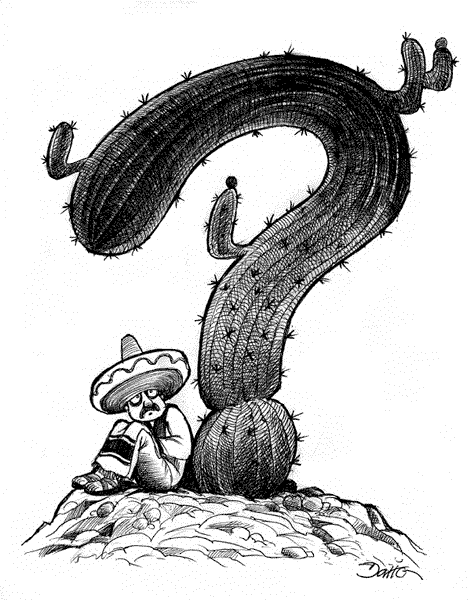
\includegraphics[width=0.5\textwidth,height=\textheight]{./pictures/textkriterien_2.png}


\includegraphics[width=0.5\textwidth,height=\textheight]{./pictures/textkriterien_5.jpg}

Welche \emph{Eigenschaften} machen Texte \emph{spezifisch}, so dass Sie
nicht beliebig füreinander austauschbar sind und eine verschiedene
Interpretation notwendig machen?

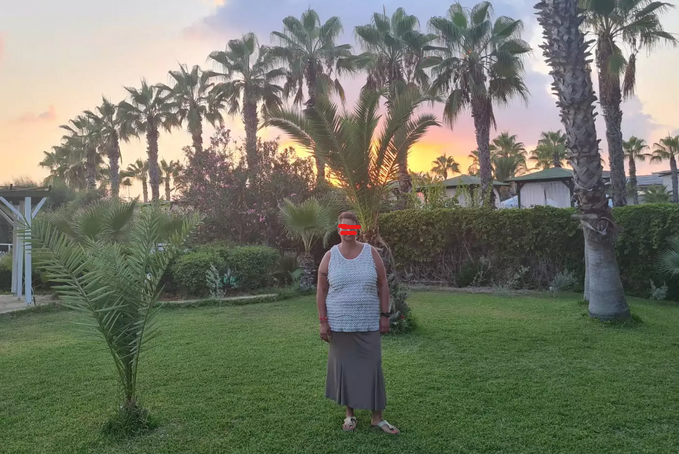
\includegraphics[width=2.26in,height=\textheight]{./pictures/partnerschaftsanzeige.png}

Ich bin 50 Jahre, 172 groß und paar kg mehr. Ich suche einen Ehrlichen,
Treuen, Zufährlässlichen Partner (keine Affären oder Ons) Er sollte 50
bis 58 sein. Bitte nur ernstgemeinte Anfragen.

Brigitte\\
Standort 1110 Wien, Simmering\\
Ad-ID: 263214\\
Zuletzt aktualisiert: 18.09.2022 14:55

\begin{center}\rule{0.5\linewidth}{0.5pt}\end{center}

Merkel-Porträt aus dem Jahr 2000 \textbf{Das eiserne Mädchen} Wer das
Geheimnis von Angela Merkel ergründen will, muss mit ihr von
Krisensitzung zu Krisensitzung ziehen und dorthin gehen, wo sie
herkommt. Eine preisgekrönte Reportage aus dem Jahr 2000, wiederentdeckt
zum 70. SPIEGEL-Geburtstag. Von Alexander Osang 28.01.2017, 07.55 Uhr

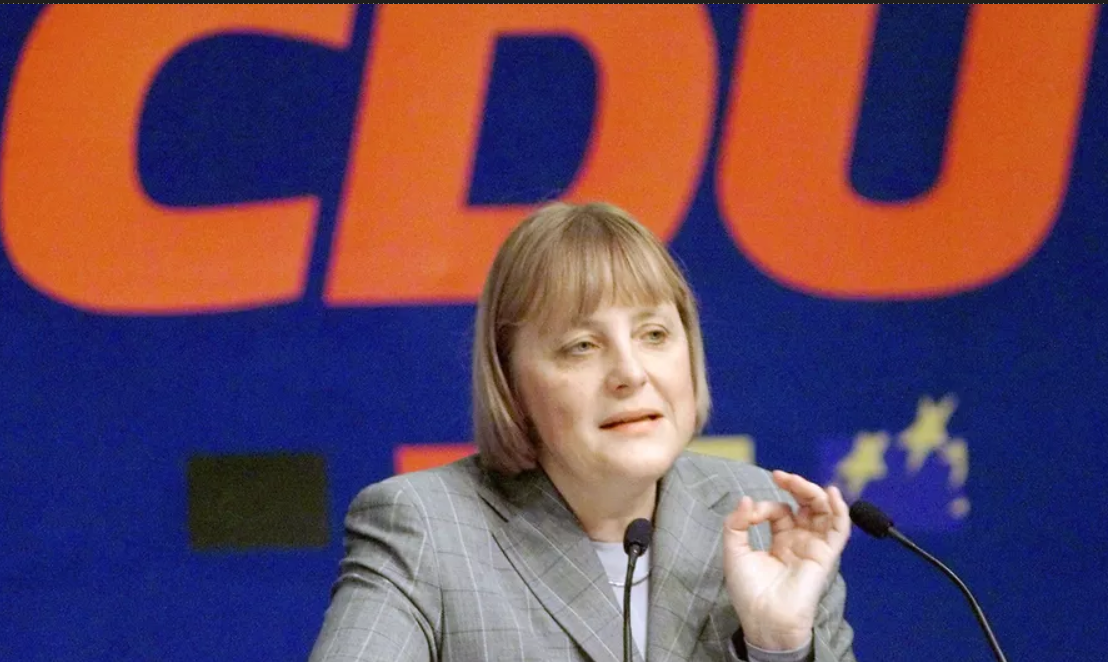
\includegraphics[width=3.69in,height=\textheight]{./pictures/Angela_Merkel_2000.png}

Manchmal muss sie noch mal zurück in diese Stadt, die so gut passt zu
Kohls Ehrenwort, zu Weyrauchs verrostetem Garagentor, zu Leisler Kieps
Einstecktuch, zu Kanthers Frisur, noch mal zurück in dieses Bonner
Konrad-Adenauer-Haus, wo man einen dieser Siebziger-Jahre-Sexfilme
drehen könnte, ohne ein einziges Möbelstück zu verrücken. Nach der
Pressekonferenz will sie schnell weg, schnell nach Berlin, der Rückflug
ist ausgebucht, alle sind in der Maschine, nur sie steht noch im
Warteraum und telefoniert. Sie weiß, in einer Stunde, in Berlin, kann
alles anders sein. Sie hört, dass Kohl heute abend im Fernsehen spricht.
Sie schaltet ihr Handy ab und sagt leise: ``Er schlägt zurück. Heute
schlägt er zurück.''

Am Abend sieht Angela Merkel Helmut Kohl im Fernsehen. Sie ist zu Besuch
bei Freunden und fragt, ob die was dagegen haben. Nein, denn Kohl gucken
gehört inzwischen dazu. Es ist spannend. Kohl marschiert in das
ZDF-Studio wie ein General. Thomas Bellut vom ZDF knallt die Hacken
zusammen. Er fragt nach Angela Merkel.

Er sei nicht hierher gekommen, um über Angela Merkel zu reden, sagt
Kohl. Und dann redet er. Wie ein betrogener Liebhaber. Oder ein
enttäuschter Vater.

Die Tür öffnet sich am Rande von Templin, es ist die Tür des letzten
Hauses in einer kurzen Sackgasse. Horst Kasner ist überraschend groß und
überraschend aufrecht für einen 74-jährigen Pfarrer. Er trägt ein graues
Cordjeans-Hemd, hat breite Schultern, aber sein linkes Auge ist trübe.
Als ich anbiete, die Schuhe auszuziehen, lacht er. Man erkennt jetzt die
Tochter in seinen Zügen. Auch die Art, wie er die Arme schwingt,
vorfreudig irgendwie, könnte sie von ihm geerbt haben. Die Frage ist,
worauf er sich freut. \ldots{} \ldots{}

\url{https://www.spiegel.de/geschichte/angela-merkel-portraet-aus-dem-jahr-2000-das-eiserne-maedchen-a-1131489.html}\footnote{Weitere
  Spiegel-Reportagen:
  \url{https://www.spiegel.de/reise/fernweh/bangkok-was-die-demonstrationen-fuer-touristen-bedeuten-a-943253.html},
  \url{https://www.spiegel.de/auto/aktuell/finale-in-le-mans-motorrad-langstrecken-wm-2013-a-923908.html},
  \url{https://www.spiegel.de/geschichte/familie-eines-fixers-heute-setz-ich-mir-den-todesschuss-a-1144782.html}}

\hypertarget{konstitutive-kriterien-der-textualituxe4t}{%
\section{Konstitutive Kriterien der
Textualität}\label{konstitutive-kriterien-der-textualituxe4t}}

Beaugrande/Dressler (1992:12ff) unterscheiden sieben konstitutive
Textualitätskriterien, die bei jedem Text erfüllt sein müssen.

\textbf{Textzentrierte} Kriterien:\\
- Kohäsion\\
- Kohärenz.

\textbf{Verwenderzentrierte} Kriterien:\\
- Intentionalität\\
- Akzeptabilität\\
- Informativität\\
- Situationalität\\
- Intertextualität.

\hypertarget{kohuxe4sion}{%
\subsection{Kohäsion}\label{kohuxe4sion}}

Dieses Merkmal reflektiert die Zusammengehörigkeit von
Oberflächeneinheiten eines Textes und beruht auf grammatischen
Abhängigkeiten.

\begin{enumerate}
\def\labelenumi{(\arabic{enumi})}
\setcounter{enumi}{1}
\tightlist
\item
  Paul hat angerufen. Er sagt, er kommt morgen.\\
\item
  A: Ich liebe dich. - B: Ich dich auch.\\
\item
  Paul hat angerufen. Paul war sehr aufgeregt.\\
\item
  O Grab ! o Wundergrab! dem alle Gräber weichen! \ldots{}\\
  O Grab! das einst begrub die Leiche aller Leichen!\\
  (Ausschnitt aus Das unbegreifliche Jesusgrab von Quirinus Kuhlmann)\\
\item
  Brüderchen und Schwesterchen\\
\item
  Kahn kritisierte seinen Chef. Er wurde entlassen.\\
\item
  Kahn kritisierte seinen Chef. Deshalb wurde er entlassen.\\
\item
  Kahn kritisierte seinen Chef. Danach wurde er entlassen.\\
\end{enumerate}

\hypertarget{kohuxe4renz}{%
\subsection{Kohärenz}\label{kohuxe4renz}}

Kohärenz = Kontinuität des Inhalts, inhaltliche Zusammengehörigkeit von
Textteilen.

\begin{enumerate}
\def\labelenumi{(\arabic{enumi})}
\setcounter{enumi}{9}
\tightlist
\item
  Die Wetterlage in Europa hat sich in den vergangenen Tagen völlig
  verändert. Wie aber soll sie von wenig Geld eine Haushaltshilfe
  bezahlen? Allerdings will kein Meteorologe einen Pfennig darauf
  verwetten, daß wir nun auch von Juni an mit Sonne rechnen können.
\end{enumerate}

Kohärenz: bei de Beaugrande \& Dressler nur semantisch-kognitive
Zusammenhänge von Texten (z .B. Kausalitäts-, Zeit- und
Referenzbeziehungen).

Die Textwelt, ist ihrerseits durch eine Sinnkontinuität bestimmt: Im
Gegensatz zur Bedeutung (der Fähigkeit oder des Potentials eines
Ausdrucks, Wissen darzustellen oder zu übermitteln) bezeichnen die
beiden Autoren mit Sinn das Wissen, das tatsächlich durch die Ausdrücke
innerhalb eines Textes übermittelt wird. Die Sinnkontinuität ist
Grundlage der Kohärenz. Eine solche dem Text zugrundeliegende
Konstellation (d.~h. die Gesamtheit der einem Text zugrundeliegenden
Sinnbeziehungen) ist die Textwelt, die mit der realen Welt nicht
unbedingt übereinstimmen muss. Es handelt sich vielmehr um die vom
Sprecher, von seinem Wissen und seinen Intentionen zugrundegelegte
Textwelt.

Konzepte sind in der Psychologie bzw. Kognitionswissenschaft angenommene
Einheiten unseres Wissenssystems, die sich aufgrund von Wahrnehmung und
Erfahrung dort gebildet haben und die nicht unbedingt ein getreues
Abbild der realen Welt ergeben. Eine Diskrepanz zwischen der
Konzept-Konstellation in der Textwelt und unserem Wissen führt dazu,
dass wir keine Sinnkontinuität herstellen können. Der betreffende Text
ist für uns sinnlos. Wenn Konzepte aktiviert werden, meint man damit,
dass sie aus dem Langzeitgedächtnis in den aktiven Gedächtnisspeicher
geladen werden.

\hypertarget{intentionalituxe4t}{%
\subsection{Intentionalität}\label{intentionalituxe4t}}

I. = Einstellung (Attitüde) des Textproduzenten, einen kohäsiven und
kohärenten Text zu bilden, um damit Wissen zu verbreiten oder ein in
einem Plan angegebenes Ziel zu erreichen.

\begin{enumerate}
\def\labelenumi{(\arabic{enumi})}
\setcounter{enumi}{10}
\tightlist
\item
  George W. Bush mit einem republikanischen Senator bei einer
  Wahlkampagne:
\end{enumerate}

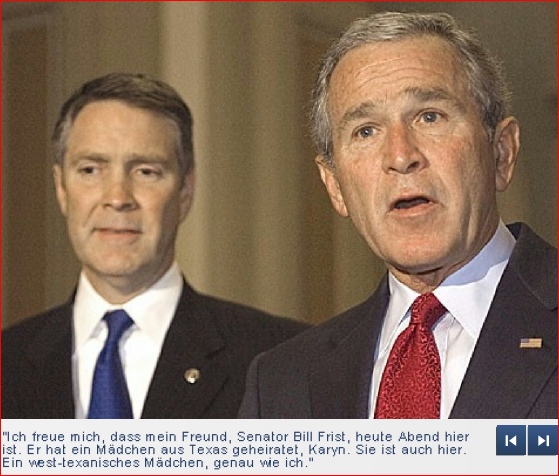
\includegraphics[width=0.75\textwidth,height=\textheight]{./pictures/textkriterien_7.png}

Widersprüche, Intentionalität als notwendiges Textualitätskriterium zu
fordern (Vater 1992: 50):\\
(a) Intentionalität: Voraussetzung für jede Art von (bewußter)
Kommunikation.\\
(b) Obwohl Kohärenz und Kohäsion unabhängige Kriterien sind und nicht
Teil eines anderen Textualitätskriteriums sein können, verweist der
Intentionalitätsbegriff auf diese beiden und macht sie zu Kriterien, die
an Intentionalität gebunden sind.\\
(c) Äußerungskomplexe, die wir intuitiv als Texte auffassen, in denen
der Textproduzent jedoch nicht Kohäsion und/oder Kohärenz intendiert.
Die Inkohärenzen der in Texten vorkommenden Sprecher stört nicht die
Kohärenz des Gesamttextes, sondern können sogar dazu gehören. Darin
zeigt sich die Abhängigkeit des Kohärenzbegriffs von der Textsorte.

\hypertarget{akzeptabilituxe4t}{%
\subsection{Akzeptabilität}\label{akzeptabilituxe4t}}

A. = Einstellung des Textrezipienten, einen kohäsiven und kohärenten
Text zu erwarten, der für ihn nützlich oder relevant ist. Akzeptabilität
bezieht sich außerdem auf die Angemessenheit der verwendeten
Sprachmittel, d.~h. auf Sprachvariation im weiteren Sinne.

\begin{enumerate}
\def\labelenumi{(\arabic{enumi})}
\setcounter{enumi}{11}
\tightlist
\item
  Ein alltägliches Bild in den Straßen des Ruhrgebiets: eine Mutter, ein
  Kind und Pommes Frites. Im Büdchen an der Ecke kauft die Frau Mama
  eine Portion Pommes Frites.\\
  Kind: Mamma, gib mich dat Pommes.\\
  Mutter: Du dummer Bengel ! Dat heißt: Gib mich dat Pommes, BITTE !
\end{enumerate}


\includegraphics[width=0.75\textwidth,height=\textheight]{./pictures/textkriterien_8.jpg}

\begin{enumerate}
\def\labelenumi{(\arabic{enumi})}
\setcounter{enumi}{12}
\item
  Ein Hühnerzüchter schreibt an eine landwirtschaftliche
  Forschungsstelle:\\
  ``Es geht um meine Hühner. Jeden Tag finde ich einige von ihnen mit
  dem Kopf im Sand und mit den Beinen nach oben. Was ist mit ihnen
  los?'' Nach 14 Tagen kommt die Antwort: ``Ihre Hühner sind tot.''
\item
  Gespräch in der Straßenbahn.\\
  ``Können Sie mir sagen, wie spät es ist?''\\
  ``Moment'', sagt der andere und zieht eine Banane aus der Tasche.\\
  Er wirft einen Blick darauf und sagt: ``Donnerstag.''\\
  ``Du lieber Himmel, da hätte ich ja an der vorigen Haltestelle
  Aussteigen müssen!''
\item
  Ein Schweizer, ein Schwabe und ein Berliner sitzen im Zugabteil.\\
  Der Schweizer zum Berliner: ``Sind Sie schou z'Züri gsi?''\\
  Der Berliner kann mit dem letzten Wort nichts anfangen und fragt
  zurück: ``Gsi?''\\
  Da greift der Schwabe hilfreich ein: ``Er moint gwää.''
\item
  Italiens Premier \emph{Berlusconi} über die Anhänger der Opposition
  vor der damaligen Parlamentswahl in Italien (2006):
\end{enumerate}

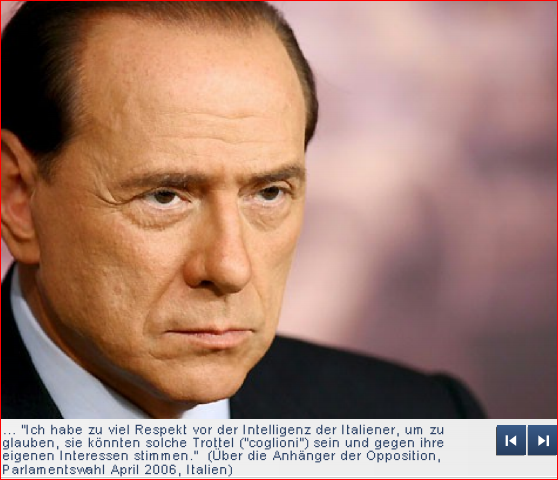
\includegraphics[width=0.75\textwidth,height=\textheight]{./pictures/textkriterien_9.png}

Einwände (Vater 1992: 52-54):\\
(a) Akzeptabilität: allgemeine Voraussetzung für erfolgreiches
Kommunizieren.\\
(b) Subjektivität: für den einen akzeptabel, für den anderen dagegen
nicht.\\
(c) Akzeptabilitätsbegriff zu eng eingegrenzt.

\hypertarget{informativituxe4t}{%
\subsection{Informativität}\label{informativituxe4t}}

I. = Ausmaß der Erwartetheit bzw. Unerwartetheit, Bekanntheit oder
Unbekanntheit, Gewissheit oder Ungewissheit der dargebotenen
Textelemente. Das richtige Maß an Informativität eines Textes ist
abhängig von Intention, Erwartung und Situation.

I. = außerdem als Thematizität verstanden. Keine athematischen Texte;
sprachlich sehr stark reduzierte Dialoge durch implizite Thematizität
gekennzeichnet sein.

\begin{enumerate}
\def\labelenumi{(\arabic{enumi})}
\setcounter{enumi}{16}
\tightlist
\item
  E = m*c2\\
\item
  um herauszufinden ob eine Konversation ein Gespräch oder eine
  Geschwätz ist, haben wir die ABC-Analyse verwendet, d.h. aufschreiben,
  ob wieviele wichtige Fachbegriffe vorkommen (welche Themen werden
  angeschnitten), wichtig hierbei ist zu schauen ob es Wörter mit Inhalt
  sind oder nur Plastikwörter und zum anderen die 4 Maximen von Grice.
  Ich hoffe das hat dich geholfen.\\
\end{enumerate}

Einwände Vater (1992: 56): Informativitätsbegriff einschränken:
Informativität sei zu definieren als das Ausmaß der Erwartetheit bzw.
Unerwartetheit von Zeichen aus einem Zeicheninventar, das dem
Rezipienten bekannt ist.

\hypertarget{situationalituxe4t}{%
\subsection{Situationalität}\label{situationalituxe4t}}

S. = Gesamtheit der Faktoren, die einen Text für eine kommunikative
Situation relevant machen.

\begin{enumerate}
\def\labelenumi{(\arabic{enumi})}
\setcounter{enumi}{18}
\tightlist
\item
  Langsam spielende Kinder\\
\item
  Die Morphologie-Vorlesung fällt heute aus.\\
\end{enumerate}

Beispiel (19) nur durch situative Faktoren interpretierbar, denn
grammatisch sind ist ein solcher Text oft nicht eindeutig. Beispiel
(20): Erwartungen von Germanistik- und Medizinstudenten bezüglich
\emph{Morphologie}-Vorlesung (Knochenbau vs.~Wortstruktur).

\hypertarget{intertextualituxe4t}{%
\subsection{Intertextualität}\label{intertextualituxe4t}}

I. = Bezug eines Textes auf andere Texte und deren Geprägtheit als
Elemente einer bestimmten Textsorte bzw. Textklasse.

Intertextualität \emph{im Sinne (a)}, d.~h. die Textsorte, ergibt sich
aus einem Geflecht verschiedener Faktoren und Merkmale: Intention, Form,
Situation usw.

Intertextualität \emph{im Sinne (b)}, d.~h. der Bezug auf andere
Textvorkommen, spielt in der Literatur (Belletristik) eine große Rolle:
z. B. Kabarett Schwarz - weiß - tot.

\hypertarget{gesamtheit-der-textualituxe4tskriterien}{%
\section{Gesamtheit der
Textualitätskriterien}\label{gesamtheit-der-textualituxe4tskriterien}}

Vater (1992: 64-66): Führt nur die Gesamtheit der Textualitätskriterien
zu Textualität, um von einem ``Text'' sprechen zu dürfen?\\
- \emph{Intentionalität} und \emph{Akzeptabilität} sind fragwürdige
Textualitätskriterien, weil sie Voraussetzung für jegliche Kommunikation
sind und nicht nur sprachlicher.\\
- \emph{Akzeptabilität} ist relativ: das gleiche sprachliche Gebilde
kann von einem Textrezipienten als Text akzeptiert werden, von einem
anderen dagegen nicht. Letzteres ist beispielsweise bei moderner Lyrik
oft der Fall.\\
- \emph{Situationalität} trägt zur Textualität bei, aber ist ein nicht
situations-adäquates sprachliches Äußerungsgeflecht kein Text? Vater
(1992: 64) scheint es in bestimmten Fällen angemessener, zu behaupten,
dass jemand zwar einen Text gebildet habe, aber halt keinen
situationsangemessenen Text.\\
- \emph{Kohäsion} ist zwar wichtig und fehlt relativ selten in Texten,
aber es gibt Äußerungsgeflechte, die durchaus ohne Kohäsionsmittel
auskommen und dennoch kohärent sein können, denn man erkennt, dass ein
Thema abgehandelt wird.\\
- \emph{Kohärenz} stellt offenbar das dominierende Textualitätskriterium
dar. Auch wenn alle anderen postulierten Kriterien nicht erfüllt sind,
kann es sich um einen Text handeln - solange das Gebilde kohärent ist.
Bestimmte Äußerungsgeflechte zeigen zudem, dass Kohärenzbeziehungen vom
Text-Thema dominiert werden.\\
- \emph{Thema}: eine nichtsprachliche Größe, die erst durch den Text
versprachlicht wird und in einen bestimmten Wissenszusammenhang
eingebettet ist. Da Textkohärenz an die Wissenssysteme des
Textproduzenten und des Textrezipienten gebunden ist, erweist es sich
als schwierig, die Textkohärenz zu bestimmen, und somit die Grenze
zwischen Text und Nicht-Text als problematisch. Kohärenz = Eigenschaft,
die an Leistungen und Urteilen von Rezipienten gebunden.\\
- \emph{Scherners Auffassung} (1984: 148), \emph{Kohärenz aufzufächern}
in:\\
(a) \emph{textbezügliche Konsistenzbedingungen} (weil ``Wörter schon
etwas mitbringen, bevor sie zur kommunikativen Verwendung gelangen'')
und\\
(b) \emph{Textbenutzer-bezogene} Kohärenzbedingungen. Die
Konsistenzbedingungen unter \emph{(a)} betreffen die
semantisch--syntaktischen Regularitäten der Vertextung, die Bedingungen
unter \emph{(b)} ``die darüber hinausgehenden Sinnerstellungsoperationen
und -voraussetzungen des jeweiligen Rezipienten'' Scherner (1984: 149;
nach Vater 1992: 66).

Kontinuum:\\
\emph{Prototypische} Texte \textless----\textgreater{}
\emph{Nicht-prototypische} Texte

\hypertarget{regulative-textprinzipien}{%
\section{Regulative Textprinzipien}\label{regulative-textprinzipien}}

Die konstitutiven Prinzipien bestimmen und erzeugen eine natürliche
Verhaltensform, die als Textkommunikation erkennbar ist. Daneben werden
von de Beaugrande \& Dressler (1992) aber auch regulative Prinzipien,
die die Textkommunikation regeln, jedoch nicht definieren: Effizienz,
Effektivität, Angemessenheit, möglicherweise noch mehrere.

\hypertarget{effizienz}{%
\subsection{Effizienz}\label{effizienz}}

Die Effizienz eines Textes steigt, wenn der Arbeitsaufwand von
Textproduzent und Textrezipient bei der Textverwendung (d.h. beim
Produzieren und beim Dekodieren) möglichst klein ist.

\hypertarget{effektivituxe4t}{%
\subsection{Effektivität}\label{effektivituxe4t}}

Die Effektivität eines Textes hängt davon ab, ob ein Text beim
Rezipienten einen starken Eindruck hinterlässt und günstige Verhältnisse
für die Erreichung eines vom Textproduzenten (und möglicherweise auch
vom Textrezipienten) angestrebten Ziels schafft.

\hypertarget{angemessenheit}{%
\subsection{Angemessenheit}\label{angemessenheit}}

Die Angemessenheit eines Textes folgt aus der Art, wie die
Textualitätskriterien in Wirklichkeit an die Situation angepasst sind.

\bookmarksetup{startatroot}

\hypertarget{abschlieuxdfende-bemerkungen}{%
\chapter{Abschließende Bemerkungen}\label{abschlieuxdfende-bemerkungen}}

Einige Hinweise für selbständige Textanalysen.

\bookmarksetup{startatroot}

\hypertarget{references}{%
\chapter*{References}\label{references}}
\addcontentsline{toc}{chapter}{References}

\hypertarget{refs}{}
\begin{CSLReferences}{1}{0}
\leavevmode\vadjust pre{\hypertarget{ref-bussmann1990lexikon}{}}%
Bußmann, Hadumod. 1990. \emph{Lexikon Der Sprachwissenschaft}. 2nd ed.
Kr{ö}ner.

\leavevmode\vadjust pre{\hypertarget{ref-eisenberg1994grundriss}{}}%
Eisenberg, Peter. 1994. \emph{Grundri{ß} Der Deutschen Grammatik}. 3.,
überarb. Aufl. Metzler.

\leavevmode\vadjust pre{\hypertarget{ref-engel1996deutsche}{}}%
Engel, Ulrich. 1996. \emph{Deutsche Grammatik. 3., Korrigierte Auflage}.
\emph{Heidelberg: Groos}.

\leavevmode\vadjust pre{\hypertarget{ref-woellstein1997satzstruktur}{}}%
Woellstein-Leisten, Angelika, Axel Heilmann, Peter Stepan, and Sten
Winkler. 1997. \emph{Deutsche Satzstruktur Grundlage Der Syntaktischen
Analyse}. Stauffenburg Verlag.

\end{CSLReferences}



\printindex

\end{document}
